\subsection{Nuclei}
    A nucleus (plural nuclei), as related to genomics, is the membrane-enclosed organelle within a cell that contains the chromosomes. The nucleus is one of the easiest organelles to detect within the cell as it is usually located in the middle and occupies a large area of the cell (\cite{Pathak_2021}, see Figure \ref{fig:cell}). The nucleus contains all of the cell's chromosomes, which in turn encode the genetic material, therefore the nucleus is an essential organelle (\cite{genomegov}). In order to stain it, DAPI was added to the cells. This is a fluorescent stain that binds strongly with some regions in DNA. DNA is strongly concentrated and near-uniformly distributed in the nucleus, hence DAPI staining identifies the nucleus (\cite{Betty_1991}). Analysis of cell's nucleus can provide many valuable insights, for example the radius of living cells is on average bigger than in the dead ones (\cite{Christiansen_2018}). With fluorescence labeling one can derive some useful features used for determining whether the well plate should or should not be selected during the selection step in the CLD process.
    %cite Christiansen 2018]  proves only success on nuclei for DIC
    \begin{figure}[htb]
        \begin{center}
            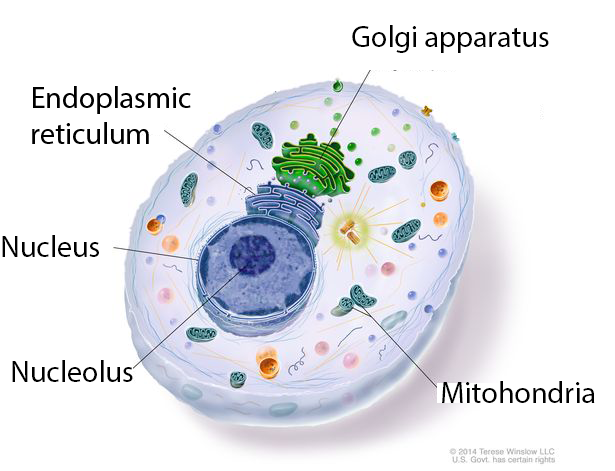
\includegraphics[width=0.4\linewidth]{bilder/cell structure.png}
            \caption[Cell structure]%
            {Cell structure. Among all organelles presented in this Figure only nucleus, endoplasmic reticulum and golgi apparatus were used and prediction targets. However, this research is easility extendable to other organelles as well. Taken from \cite{cell}}\label{fig:cell}
        \end{center}
    \end{figure}
    \subsubsection{Preprocessing}\label{section:nuclei-preprocessing}
        As not all of the dataset samples were of the same quality it was important to first manually filter the dataset to remove the bad imaging samples. Even with the normal conditions many of the images contain a lot of background. This creates a background vs. foreground class imbalance (see Figure \ref{fig:bad-smaples}a). Overexposure is also a typical problem that creates samples of a too high intensity and with details inside the nucleus missing (see Figure \ref{fig:bad-smaples}b, c). Lastly, underexposure is just as problematic as overexposure (see Figure \ref{fig:bad-smaples}d).

\begin{figure}[H]
	\begin{center}
		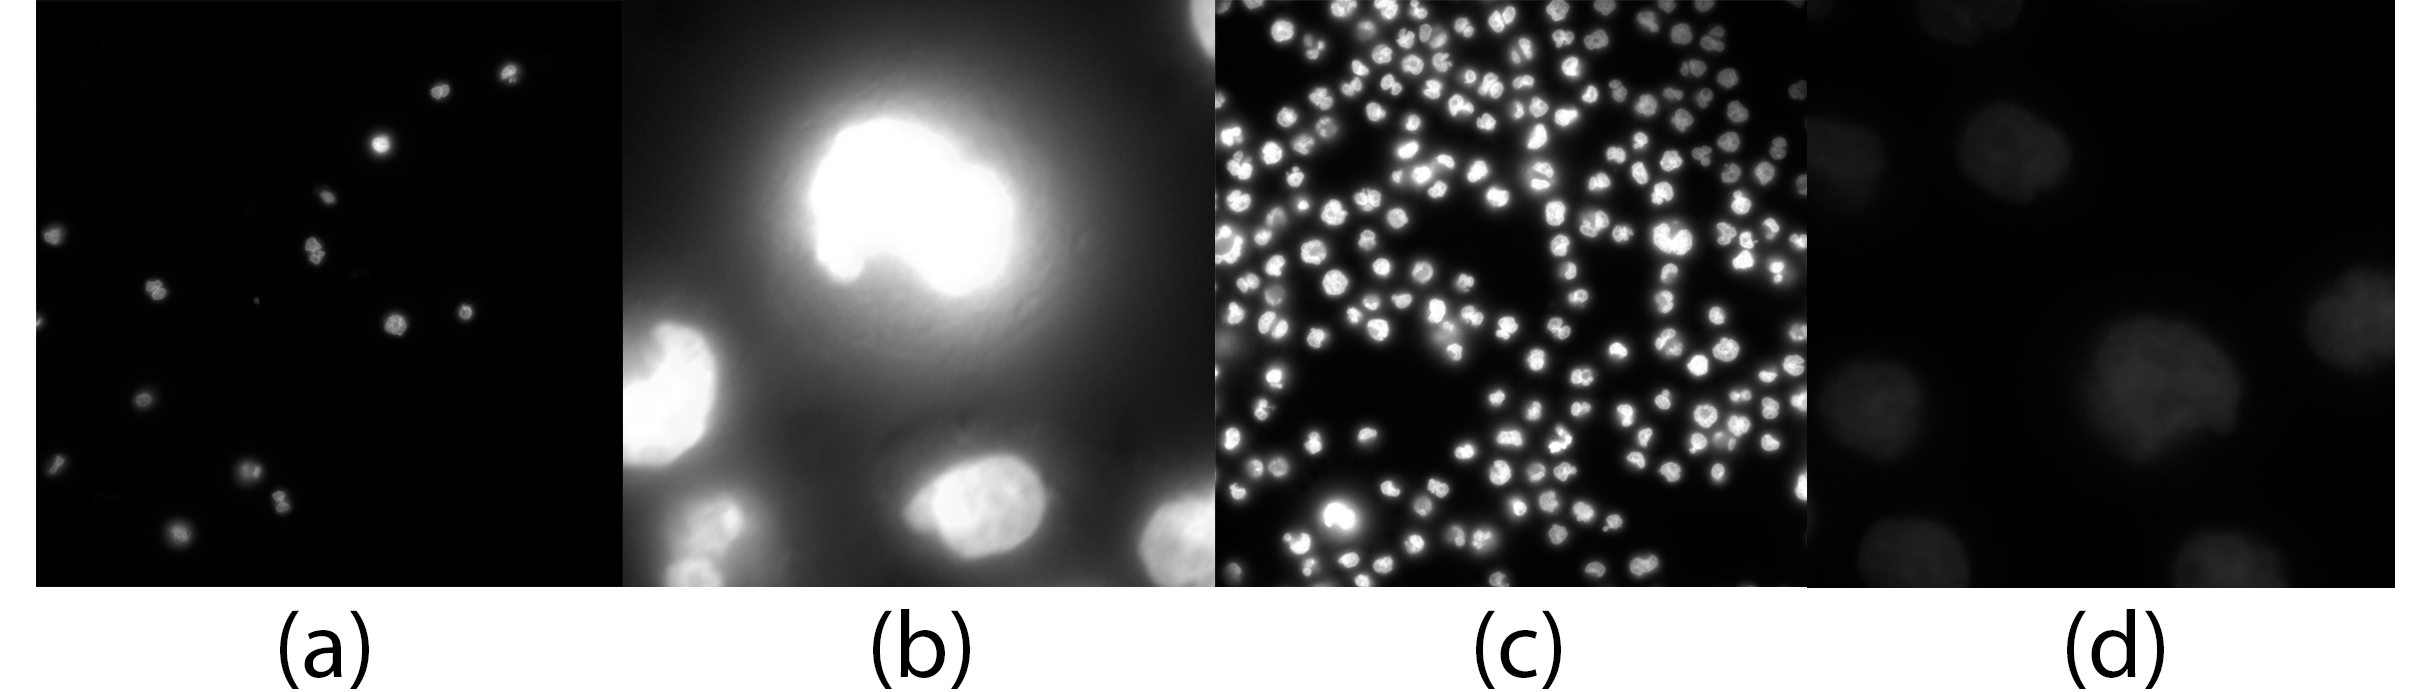
\includegraphics[width=0.7\linewidth]{bilder/nuclei/filter-out.png}
		\caption[Nuclei fluorescence samples to be filtered out]%
		{Nuclei fluorescence samples to be filtered out. (a) --- too few cells in the image result in many fully black crops; (b) --- overexposure; (c) --- overexposure, lack of details; (d) --- underexposure.}\label{fig:bad-smaples}
	\end{center}
\end{figure}

Once the images have been filtered out, they were normalized to have the values between 0 and 1.

    \subsubsection{Training and predictions}
        \paragraph{Convergence}
              %\begin{figure}[H]
%	\begin{center}
%		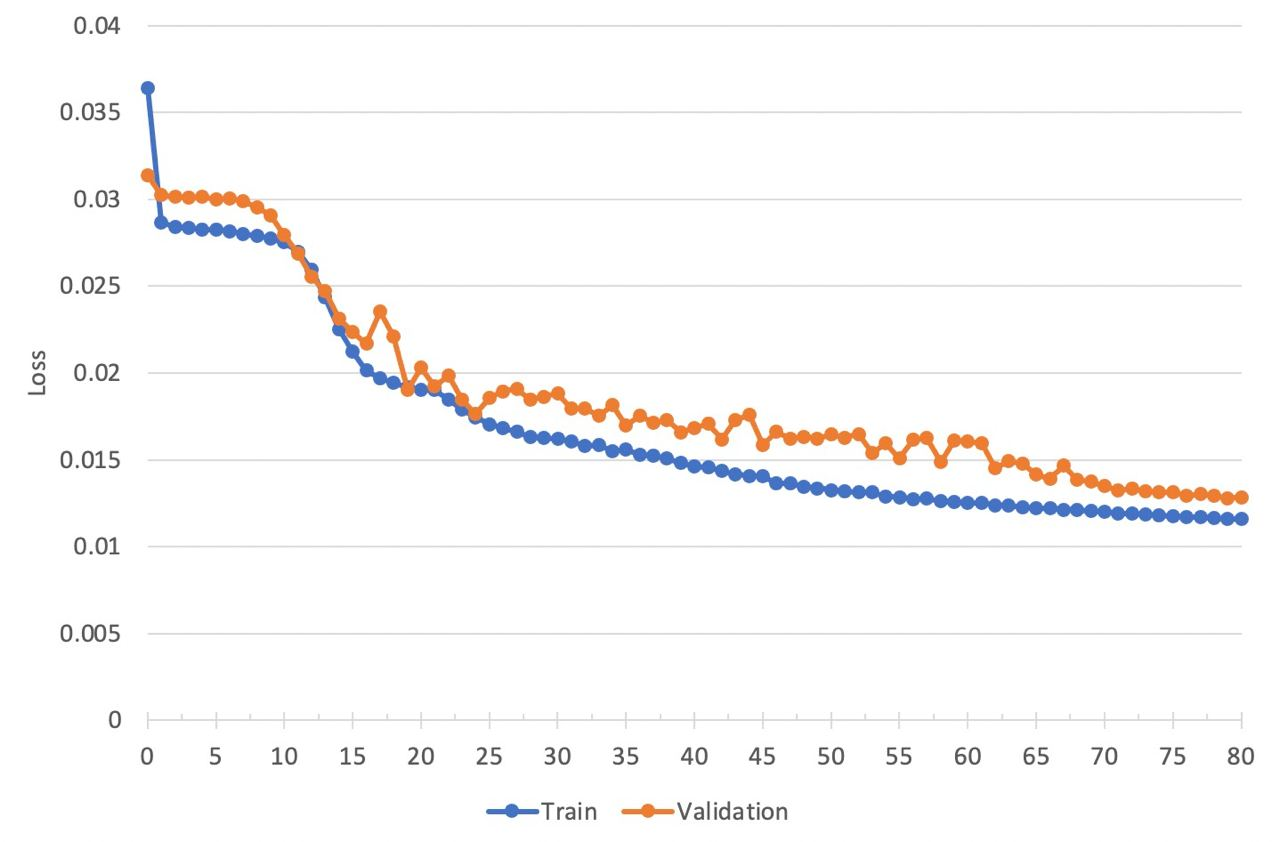
\includegraphics[width=0.5\linewidth]{bilder/nuclei/no-wi.jpg}
%		\caption{Default weight initialization is not suitable}\label{fig:no-wi}
%	\end{center}
%\end{figure}

%\begin{figure}[H]
%	\begin{center}
%		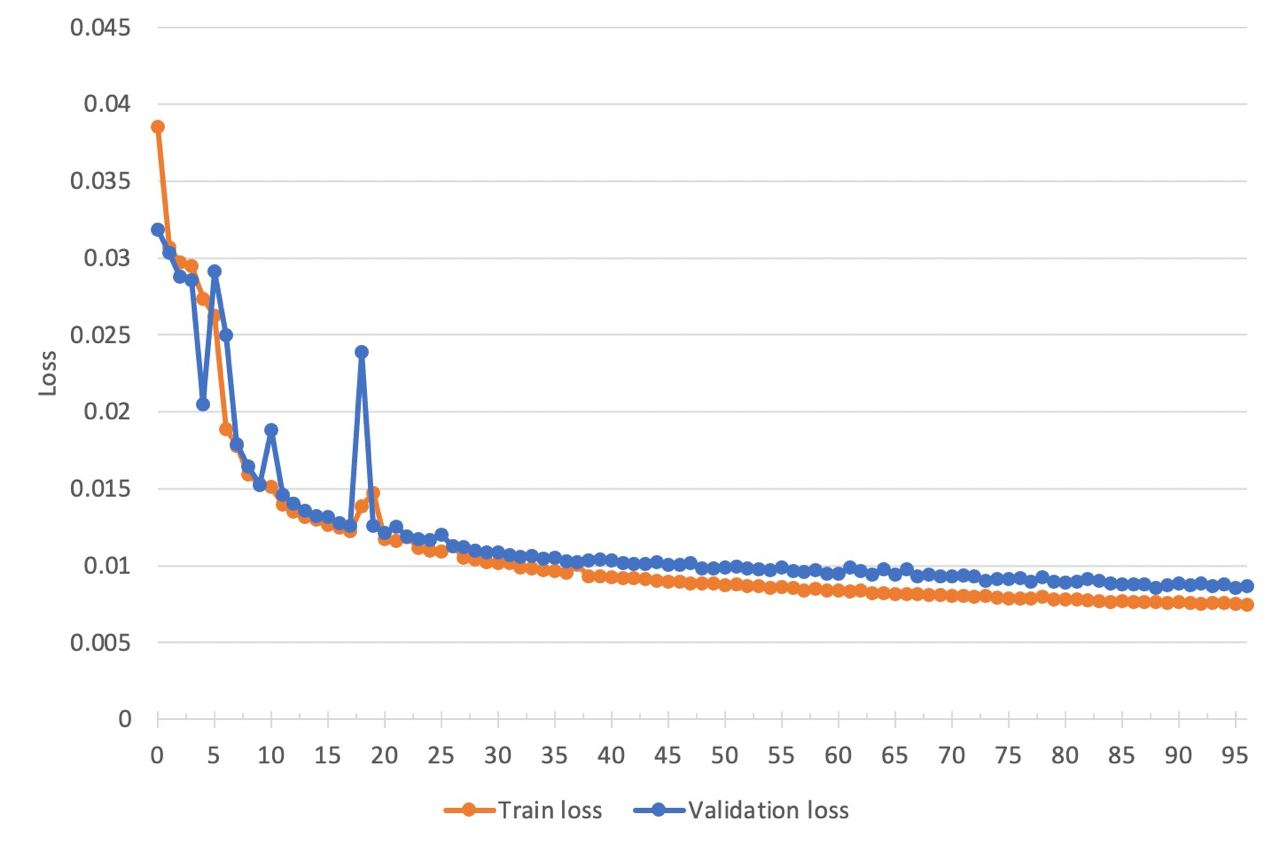
\includegraphics[width=0.5\linewidth]{bilder/nuclei/pca-2-datasets.jpg}
%		\caption{PCC with correct weight initialization converges but unstable}\label{fig:pcc-2-dataset}
%	\end{center}
%\end{figure}

As the nuclei dataset is one of the biggest ones (see Table \ref{table:data}), the experiments would first be performed on the subset of the data, and only once the training pipeline and good results were established, the training would be done using the full dataset. Figure \ref{fig:wi} (right) represents the training of nuclei using only two 96-well plates with MSE loss. The training is very unstable in the begining, but one can clearly see that the model successfully converges afterwards. Our hypothesis behind the instability was the clear lack of training data, which was proven by further training using the full data and as a result achieving a more stable PCC loss (see Figure \ref{fig:full-dataset-pcc}).

\begin{figure}[htb]
	\begin{center}
		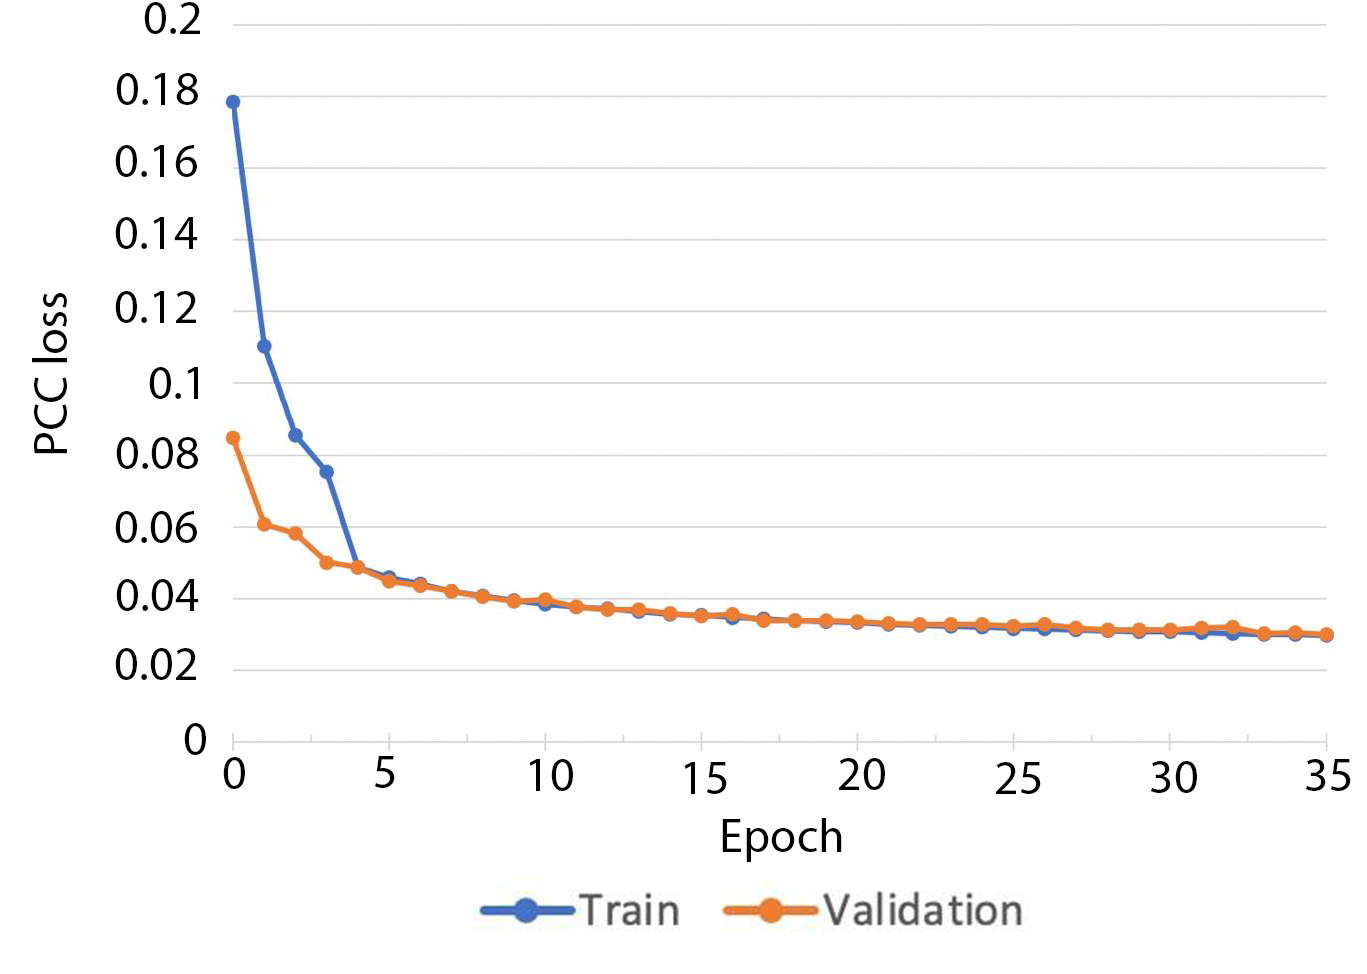
\includegraphics[width=0.5\linewidth]{bilder/nuclei/full-dataset.png}
		\caption{Having more data makes training more stable}\label{fig:full-dataset-pcc}
	\end{center}
\end{figure}

As mentioned in definition \ref{def:pcc-loss} for correct understanding of the following plots, one should be careful with differentiating PCC loss from PCC itself. PCC loss converts PCC to be between $0$ and $1$, with $0$ being an optimal value.

Seeing that the model significantly stabilizes with the use of more data and that the prediction results become much more similar to the ground truth (see Figure \ref{fig:nuclei-comparison-predictions} \textit{small dataset} vs. \textit{full dataset}), it was decided to try the use of augmentations in order to enlarge the dataset even more. In this case the augmentations were not used in order to regularize or stabilize training (by providing more difficult, for instance, blurred samples), but to simply have more data. Training and validation PCC losses from the training with the use of augmented data are presented in Figure \ref{fig:no-reg-augmented}. The augmentations used here are horizontal and vertical flips, rotations and crops (described in detail in section \ref{section:augmentations}).
\begin{figure}[H]
	\begin{center}
		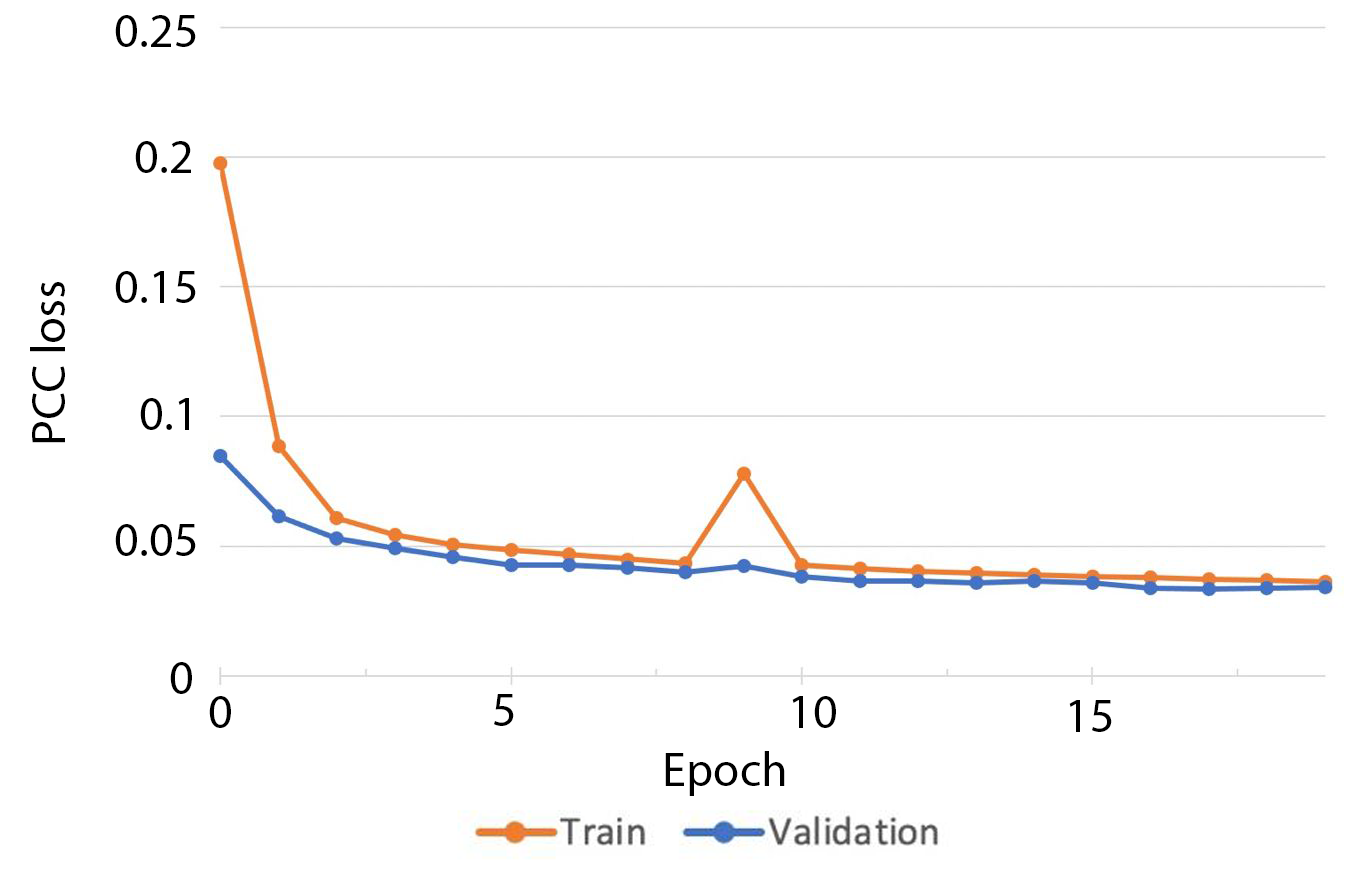
\includegraphics[width=0.5\linewidth]{bilder/nuclei/no-reg-but-aug.png}
		\caption{Adding simple augmentations in the dataset}\label{fig:no-reg-augmented}
	\end{center}
\end{figure}
Validation PCC loss has slightly increased to $0.0381$ in comparison to the previous value of $0.0365$. However, the validation set on which this loss was estimated also includes augmentations mentioned above and therefore presents a slightly more difficult task than the original validation set. True improvement is confirmed by measuring the loss of the models on the same dataset, where PCC loss has improved from $0.0365$ to $0.0322$ (or PCC from $0.92$ to $0.93$).

In the next experiment the model has additionally been regularized by adding dropout layers and using a weight decay of $0.0001$ (see Figure \ref{fig:full-dataset-pcc-regularized}). This did not bring a better result, but has only made it more difficult for the model to capture the needed feature to reproduce the fine details within the nuclei. However, this brought up a new hypothesis, namely that the model might simply have not enough of capacity to capture enough of the details. In order to confirm this a bigger model has to be trained.
\begin{figure}[htb]
	\begin{center}
		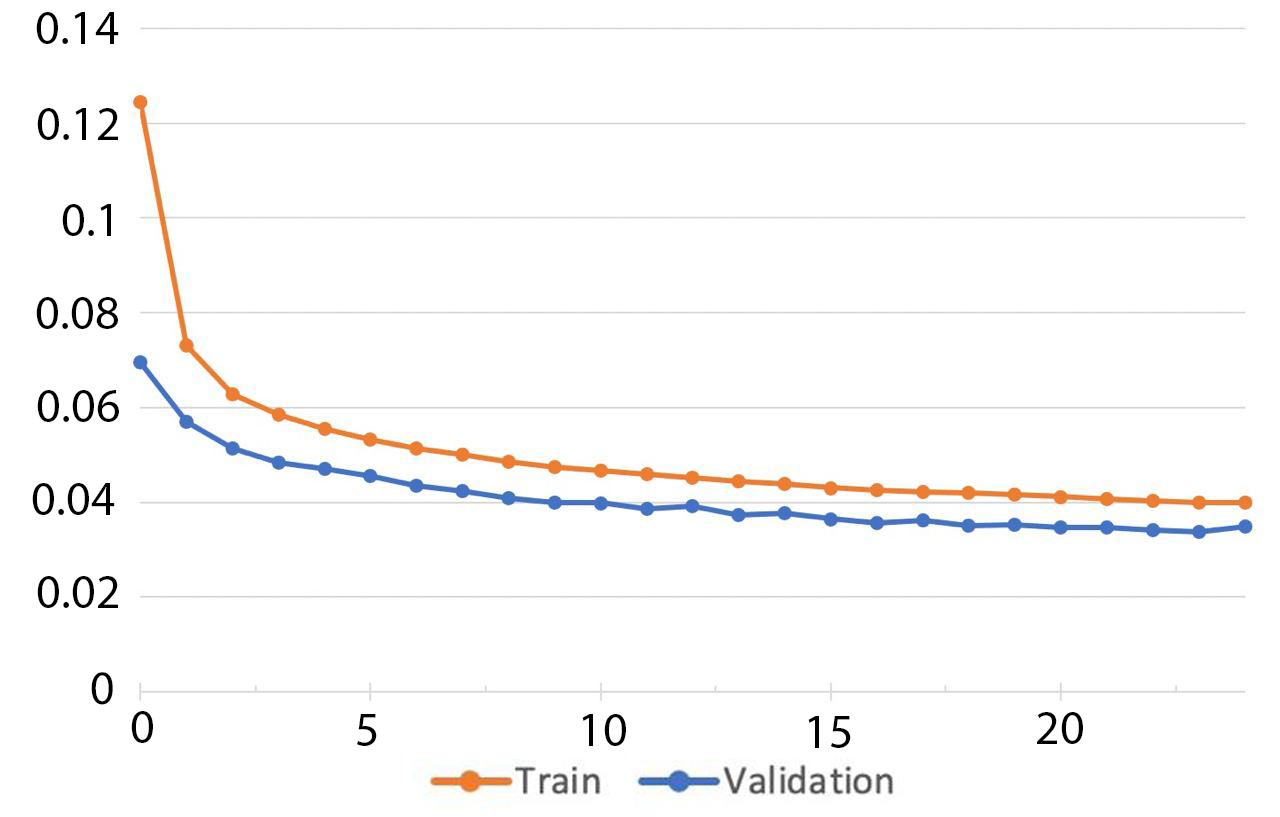
\includegraphics[width=0.5\linewidth]{bilder/nuclei/full-dataset-regularized.png}
		\caption{With regularization and augmentations}\label{fig:full-dataset-pcc-regularized}
	\end{center}
\end{figure}

\begin{figure}[htb]
	\begin{center}
		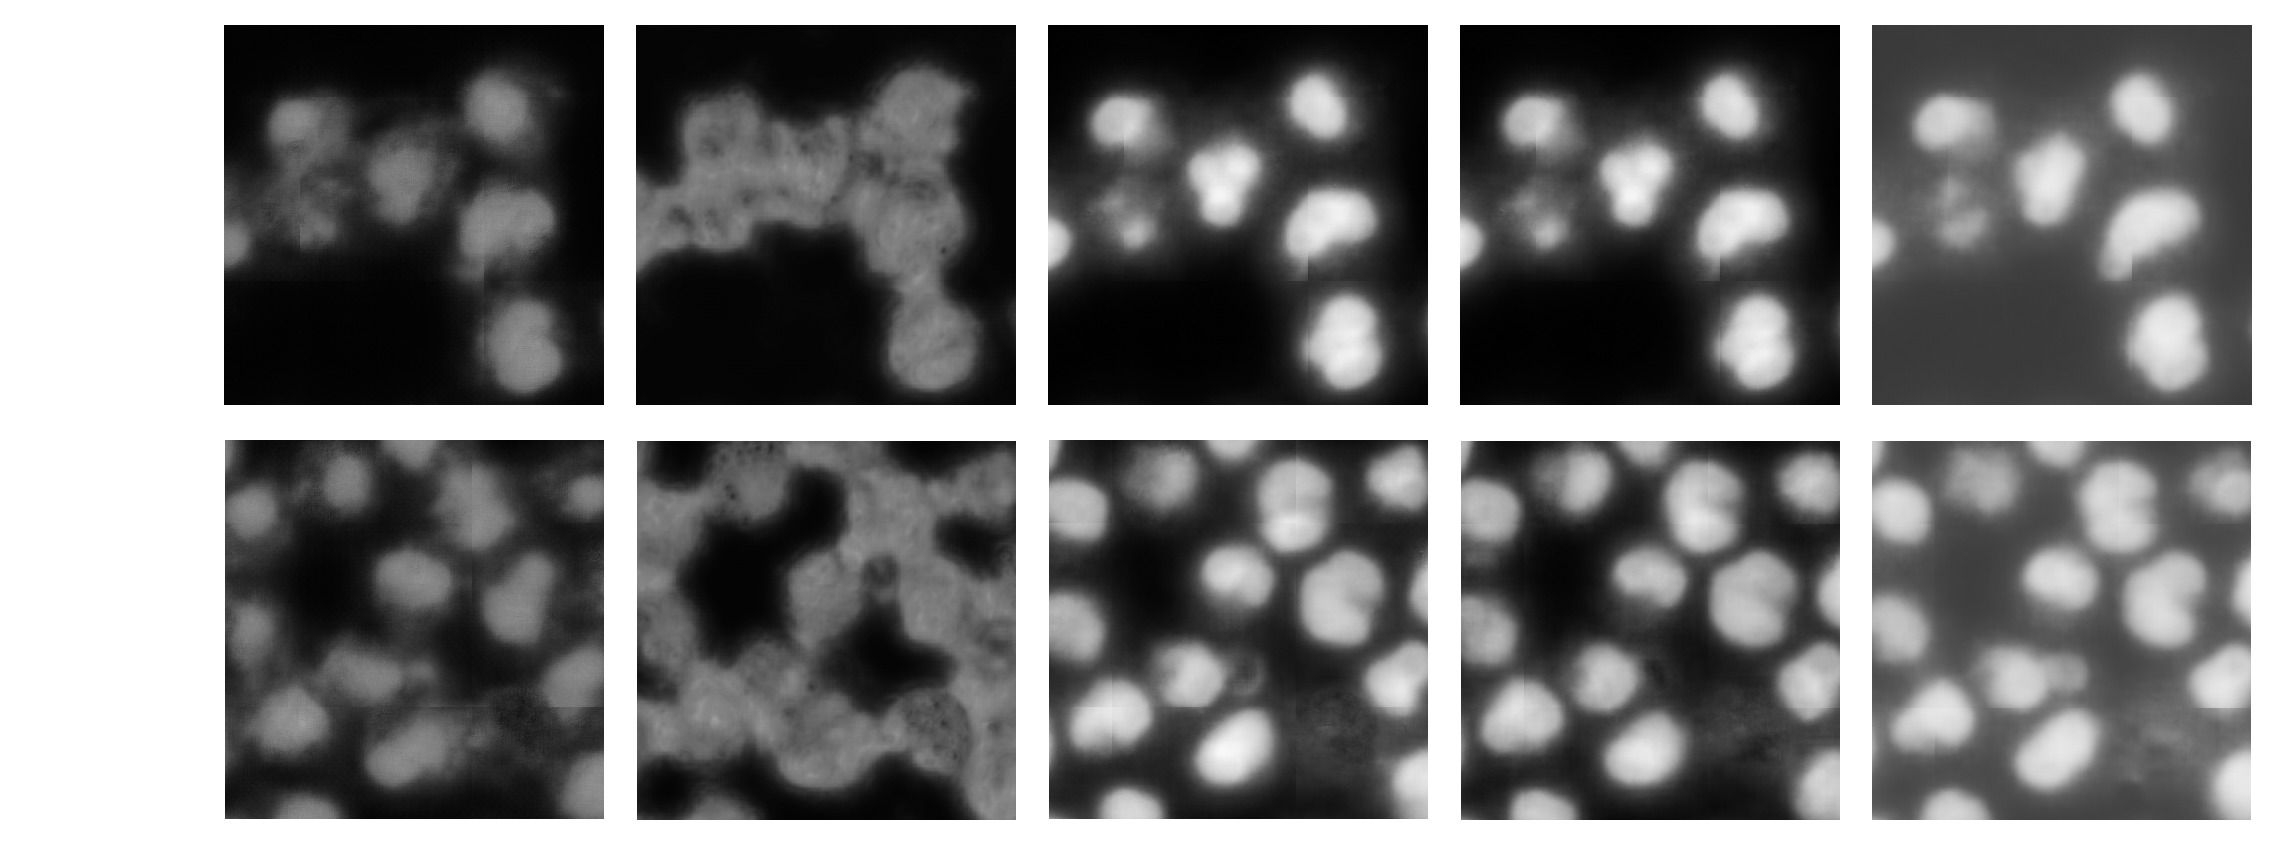
\includegraphics[width=0.6\linewidth]{bilder/nuclei/comparison-chzn-phx.png}
		\caption[Comparison of different models predictions and scores]%
		{Comparison of different models predictions and scores. PCC loss is representative of predictions quality, whereas MSE loss is not. Increasing model's size significantly improves the results.}\label{fig:nuclei-comparison-predictions}
	\end{center}
\end{figure}

Interestigly observations made in this section made it clear that metrics used for training (PCC and MSE losses) are indeed not representative enough to derive any conclusions regarding the model quality from them. Just by looking at Figure \ref{fig:nuclei-comparison-predictions} one can see that for example, training on the full dataset of data gives much better results than training on the small dataset. Yet MSE seems to be bigger for this experiment. Also, it is not representative in comparison of a model without the correct weight initialization vs. the regularized model with augmentations. MSE loss is much higher there, because in general the image became somewhat brighter, even though the quality of the nuclei is significantly better. PCC loss seems to represent the desired quality of the model better. This trend has been noticed by \cite{Lachance_2020} as well. They state that values of PCC lack the practical context --- which value would be good enough and good enough in which context? This issue has been addressed here as well in section \ref{section:model-evaluation}, where more practical metrics are introduced and the model evaluation on them is carried out.

        \paragraph{Prediction quality}
            \label{section:nuclei-predictions}
              \begin{figure}[H]
	\begin{center}
		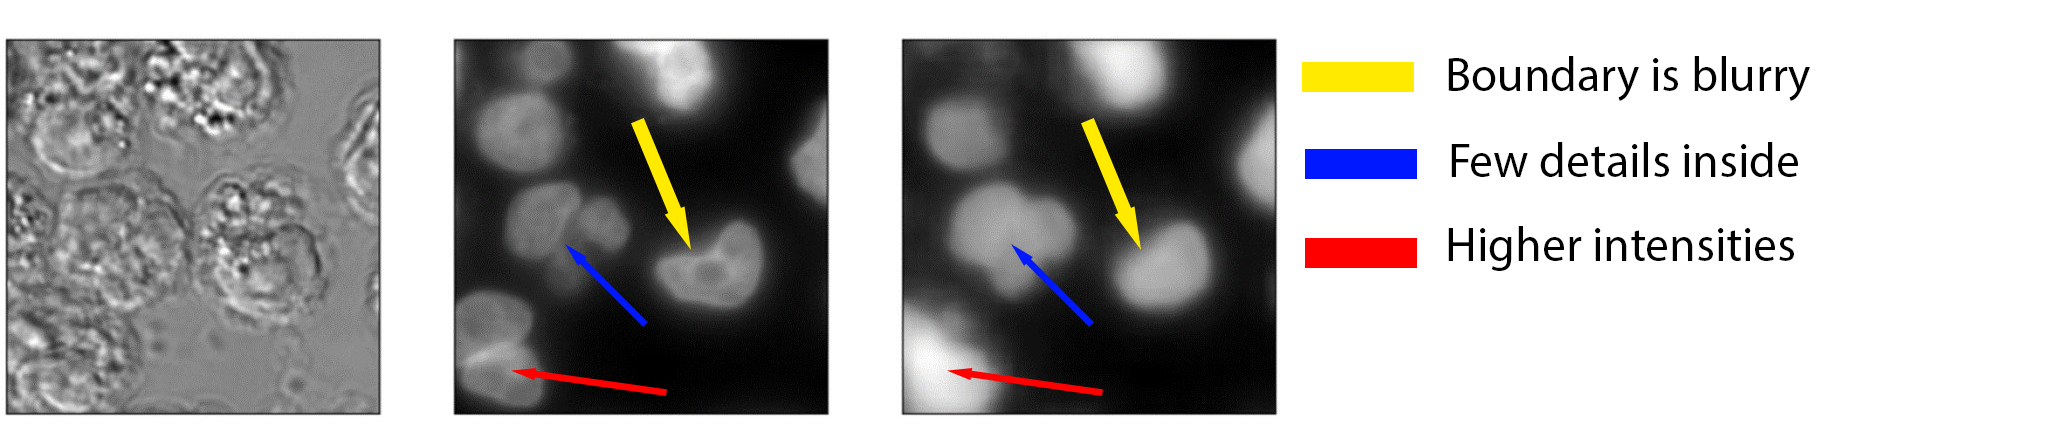
\includegraphics[width=0.8\linewidth]{bilder/nuclei/problems.png}
		\caption{Problems in predictions}\label{fig:nuclei-troubles}
	\end{center}
\end{figure}

\begin{figure}[H]
	\begin{center}
		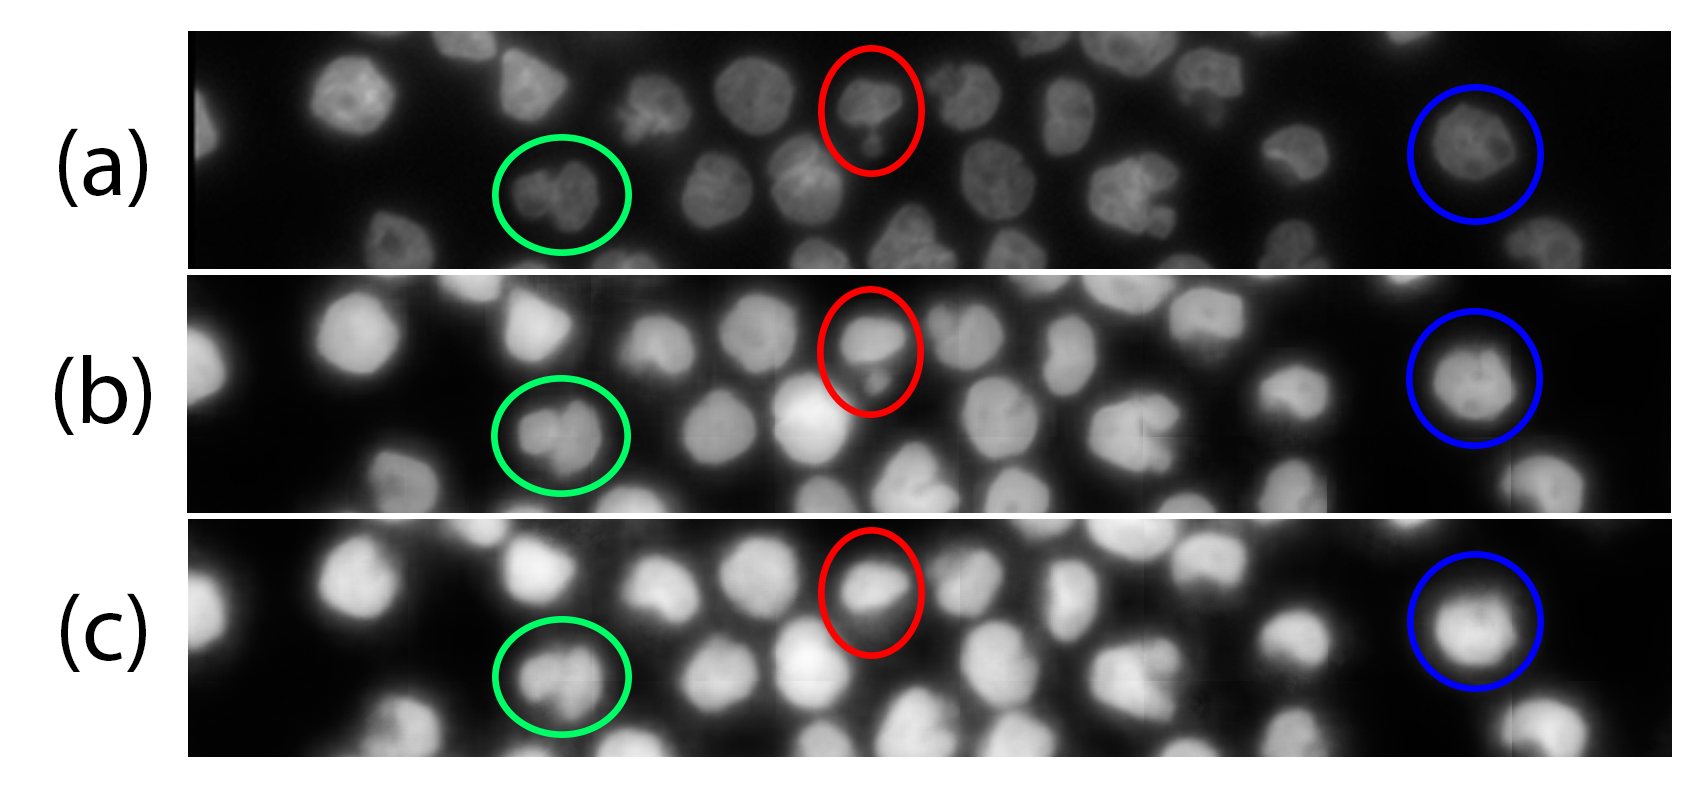
\includegraphics[width=0.6\linewidth]{bilder/nuclei/bigger-model.png}
		\caption{Predictions improvement}\label{fig:better-nuclei}
	\end{center}
\end{figure}
    \subsubsection{Postprocessing for nuclei segmentation}
        To properly evaluate the practical biological metrics described in section \ref{section:model-evaluation} on model predictions, one must be able to segment nuclei from fluorescence (as well as from predictions) first. Segmentation in this context refers to the creation of a mask. It should consist of $0$s and $1$s,  with a one being assigned to every pixel that is a part of the nucleus, while all the other ones are assigned with a zero. Although this might be a straightforward task for our eyes, it is not that easy to select separate nuclei via postprocessing. There are several edge cases where the nuclei are difficult to segment.

Even though the most extreme corruptions mentioned in section \ref{section:nuclei-preprocessing} were filtered out, some of the images that are corrupted not as severely (meaning they still have all the visible features needed for learning) are still present in the dataset, hence avoiding significant reduction of the amount of data.
\begin{figure}[H]
    \centering
    \setkeys{Gin}{width=\linewidth}
    \centering
        \begin{tabularx}{\textwidth}{YYYY}
            \textbf{Too few cells} &
            \textbf{Overexposure} &
            \textbf{Light gradient} &
            \textbf{Normal lighting} \\
            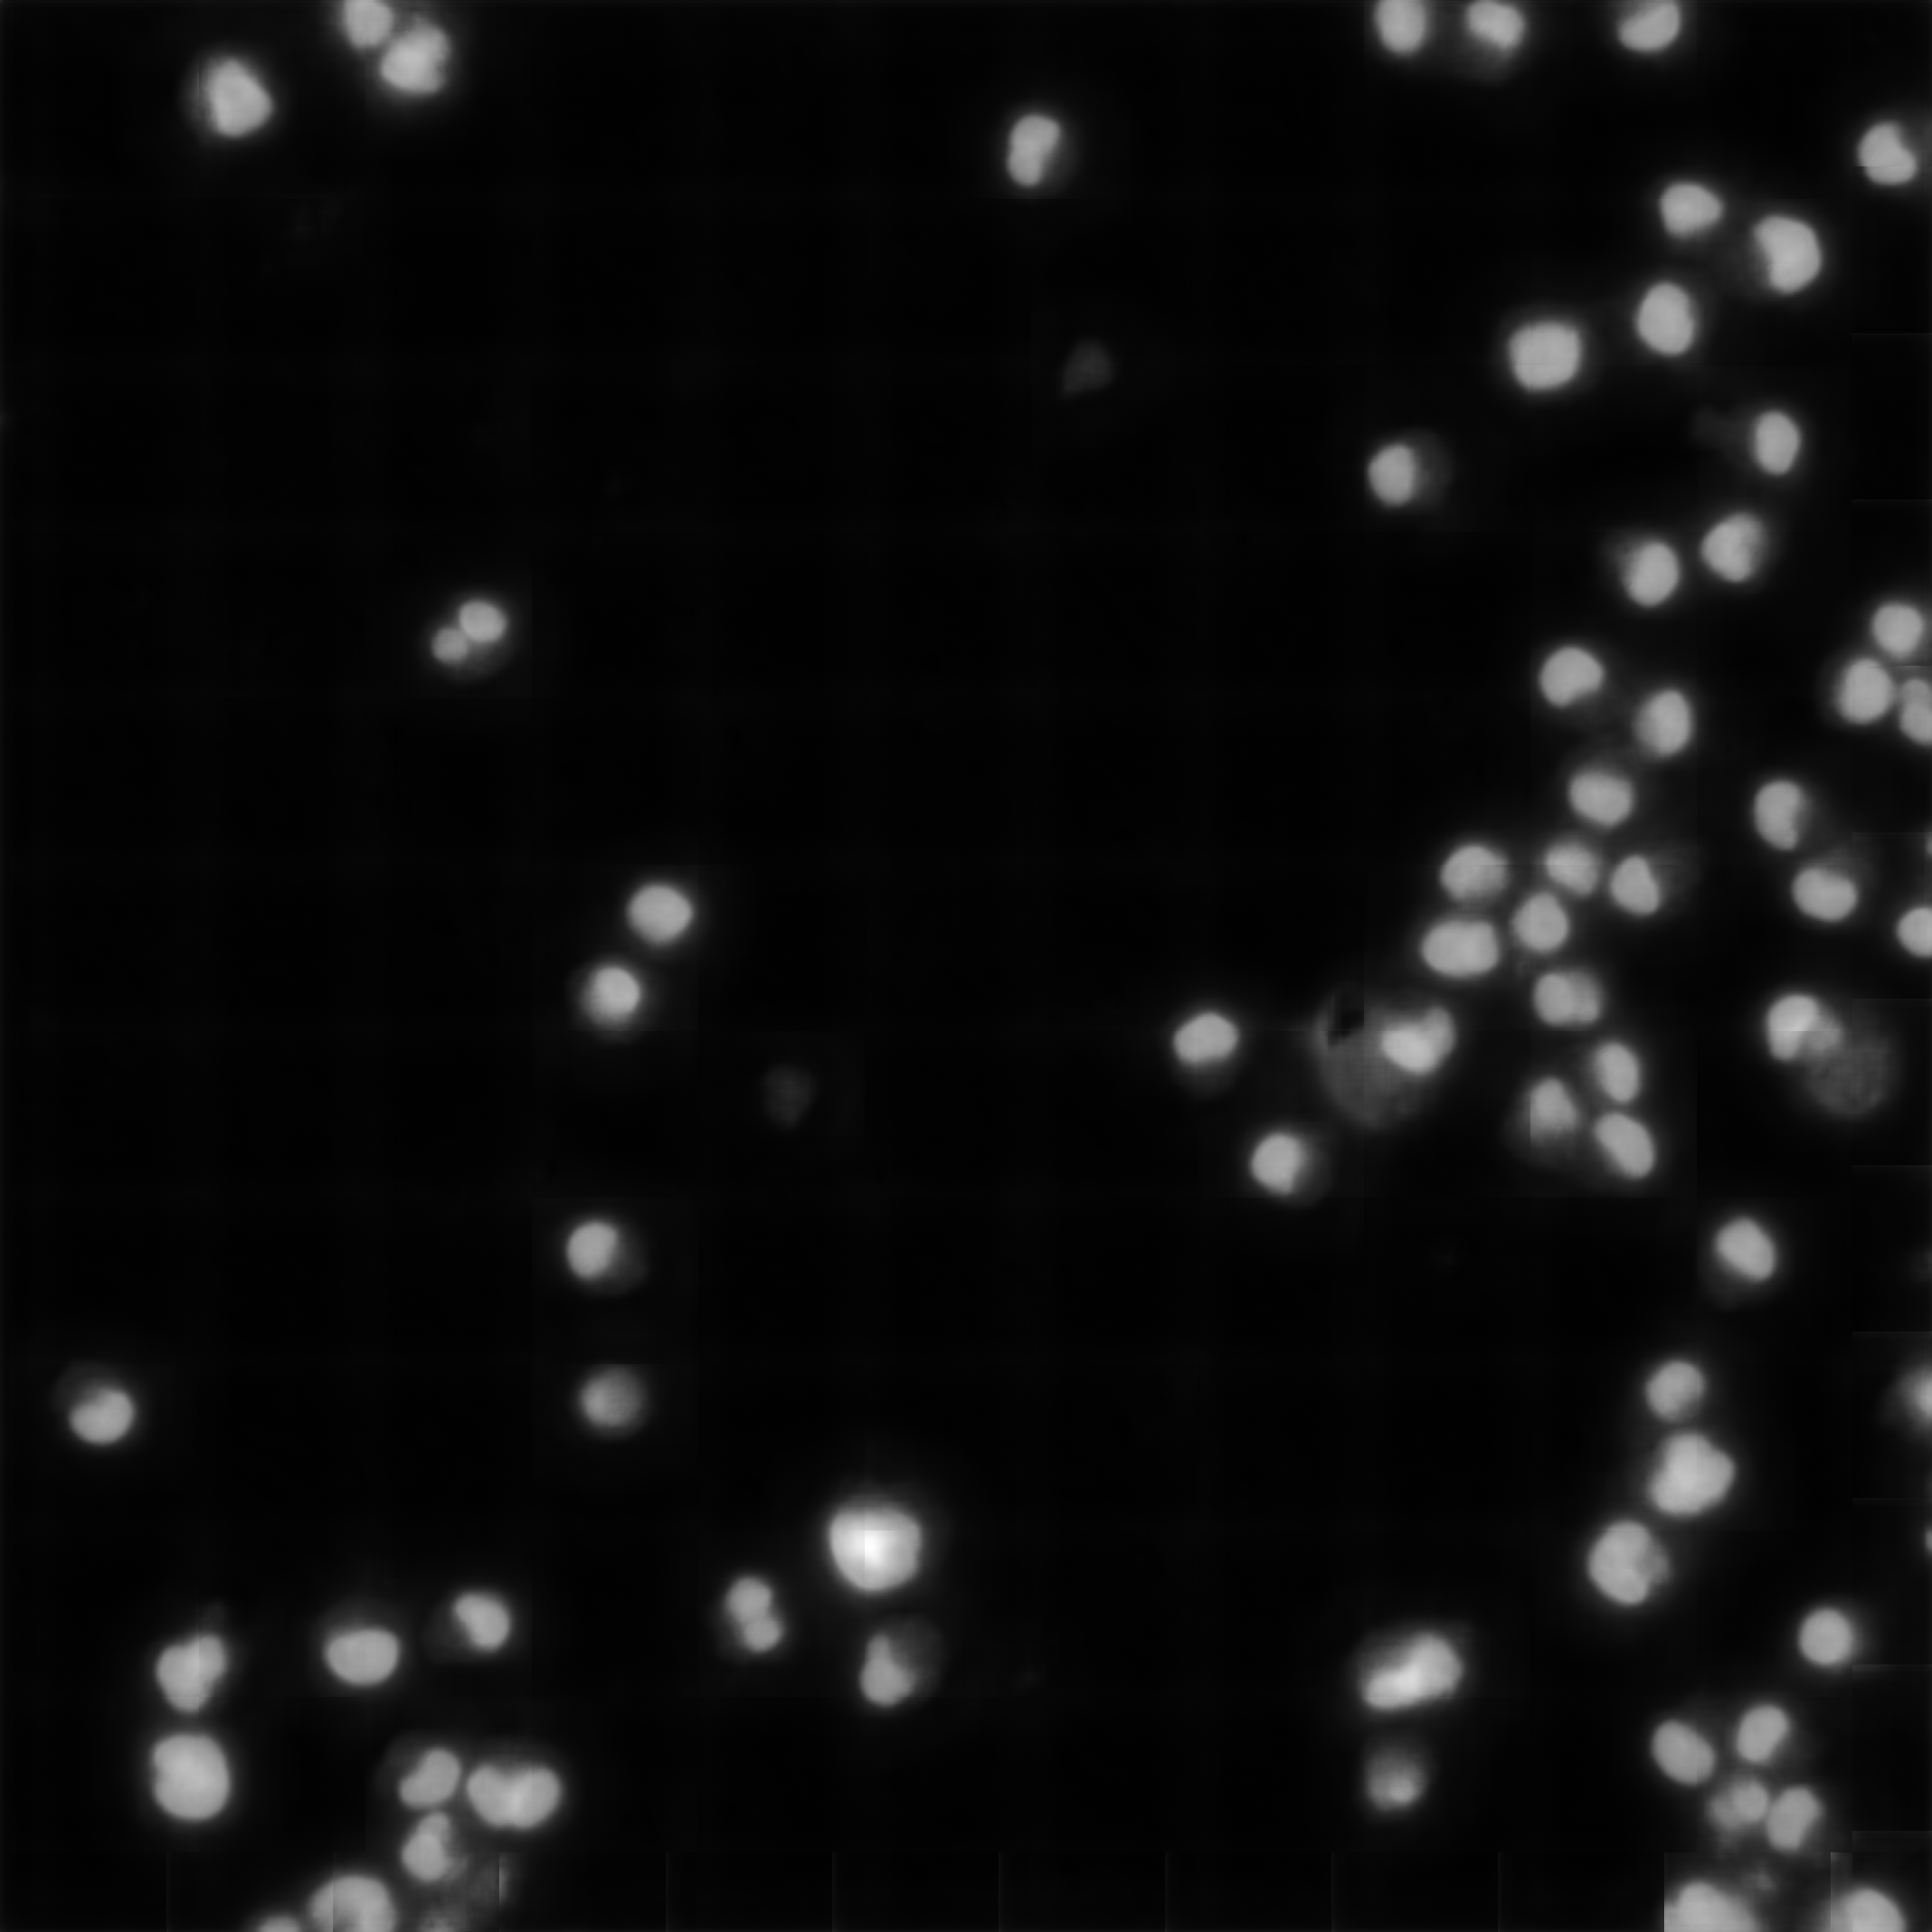
\includegraphics{bilder/lightning-conditions/lightning-1.png} & 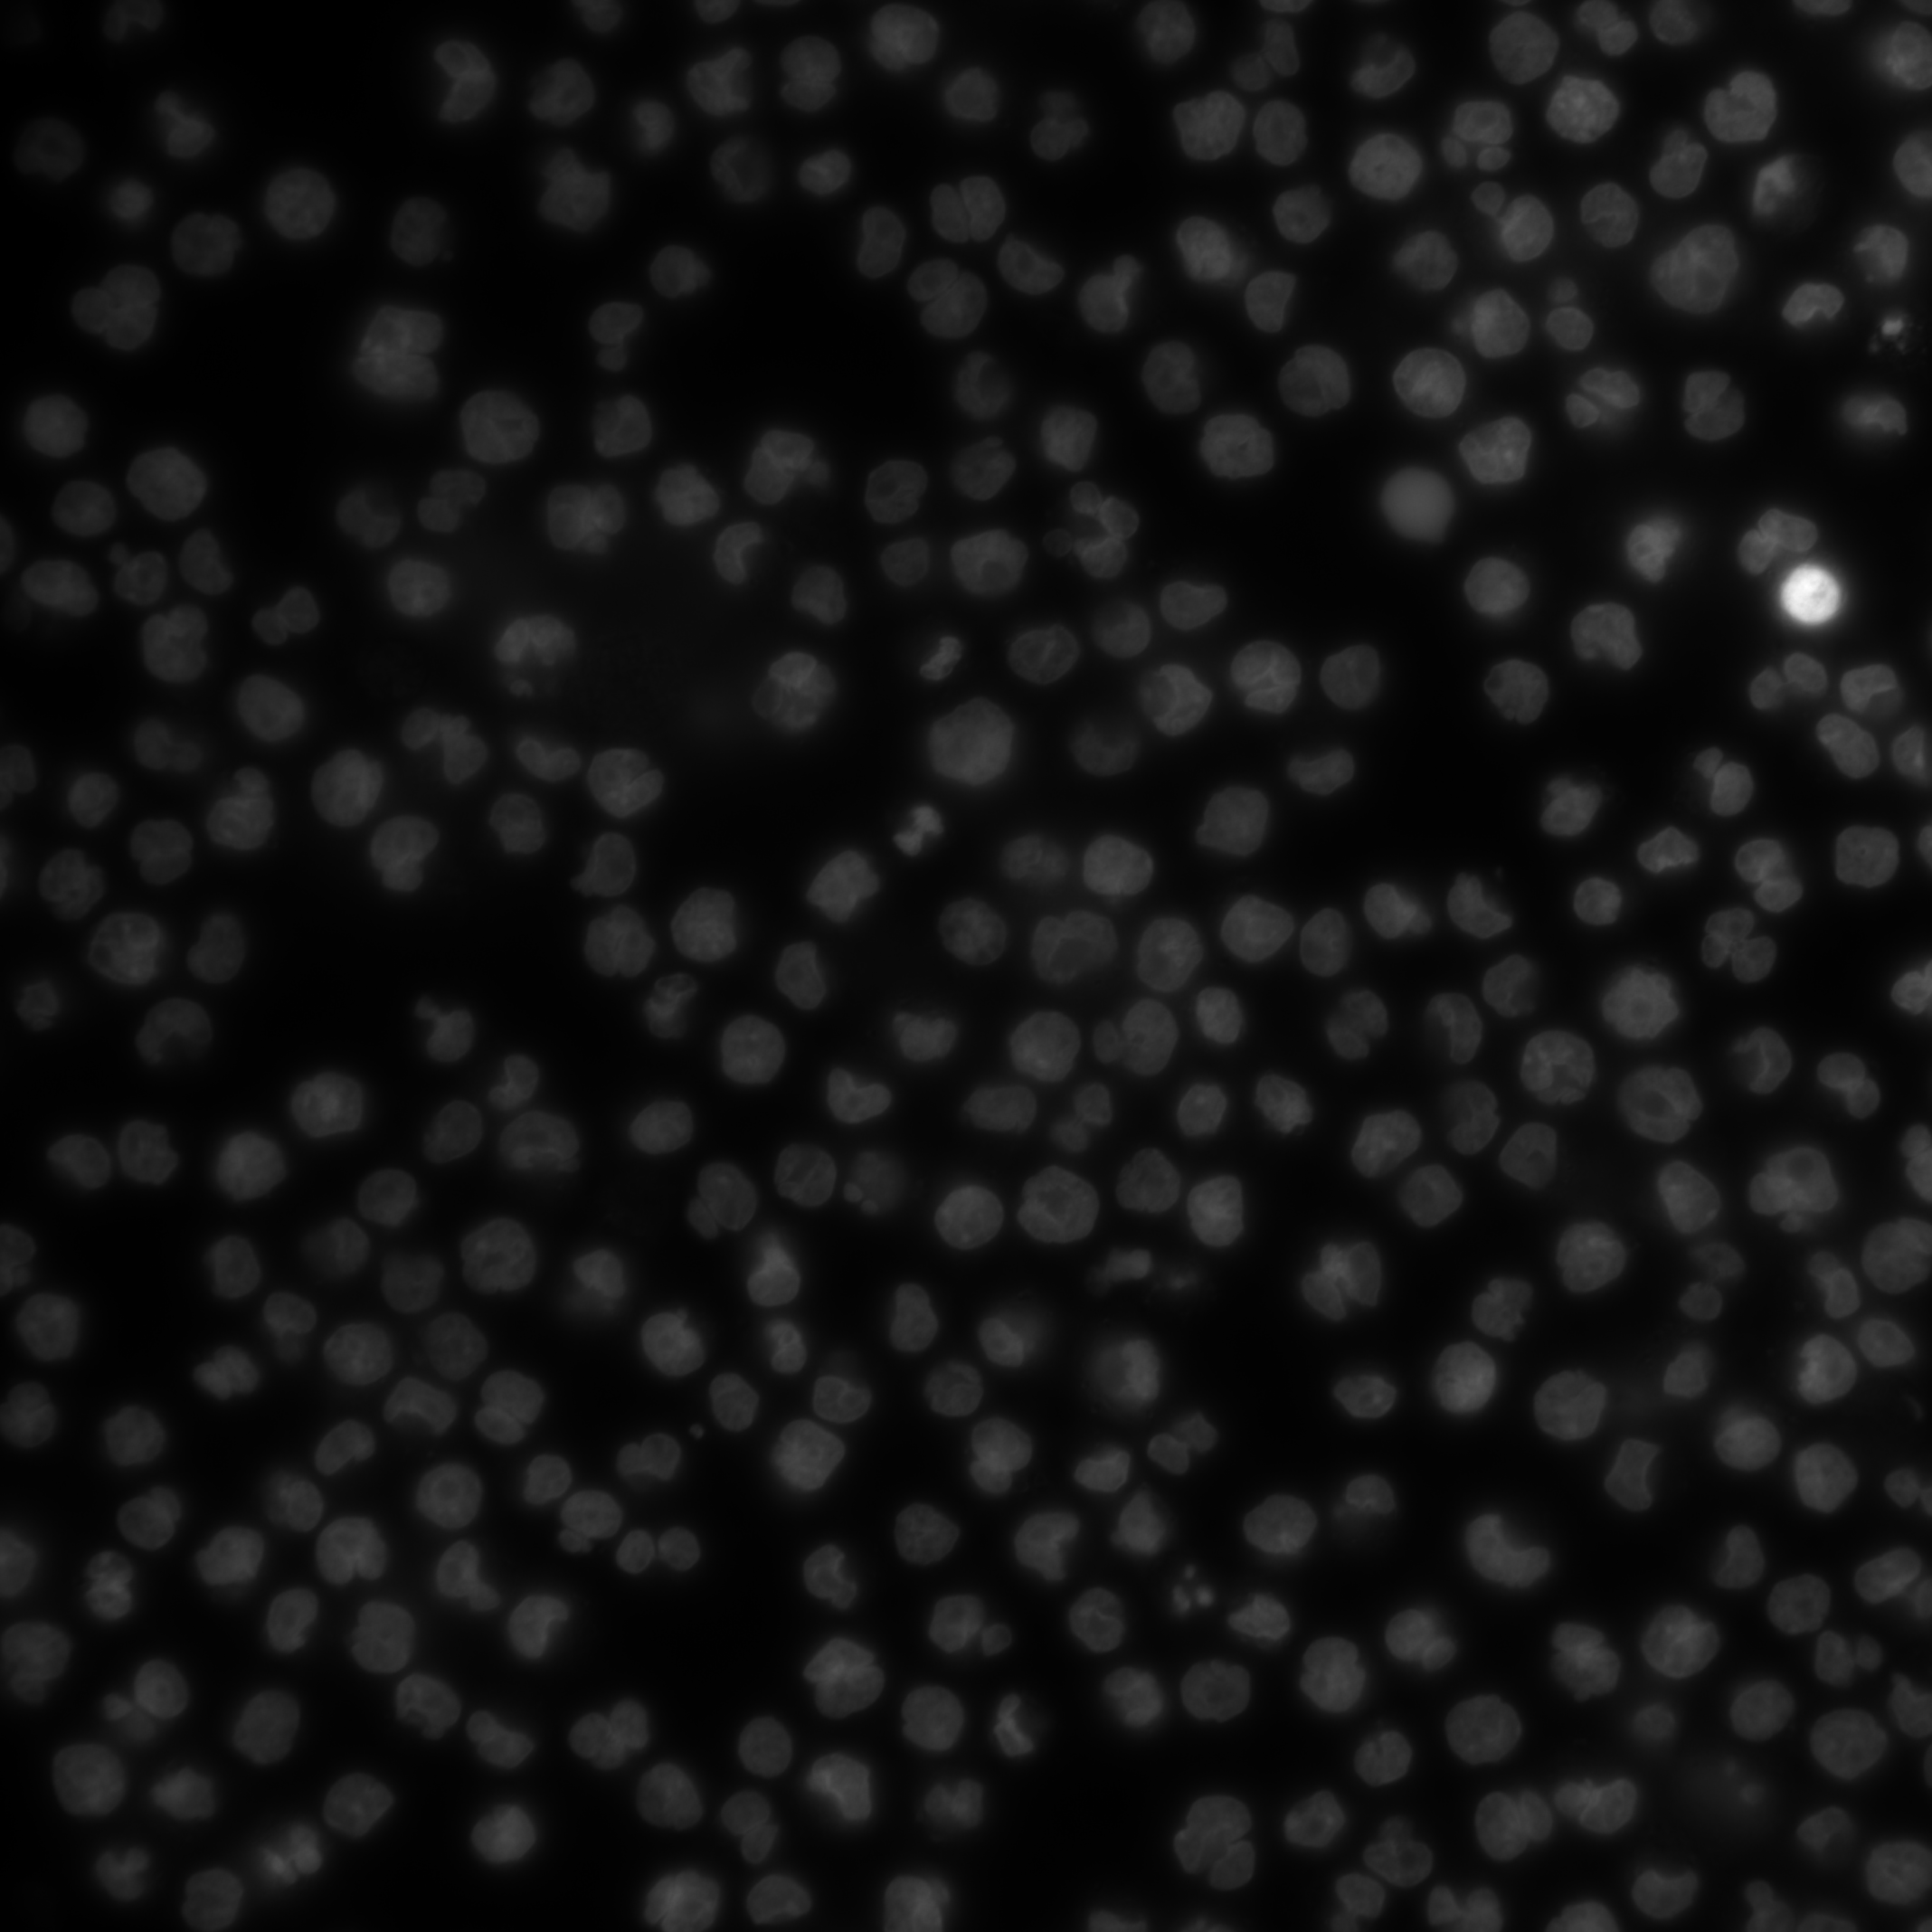
\includegraphics{bilder/lightning-conditions/lightning-2.png} &
            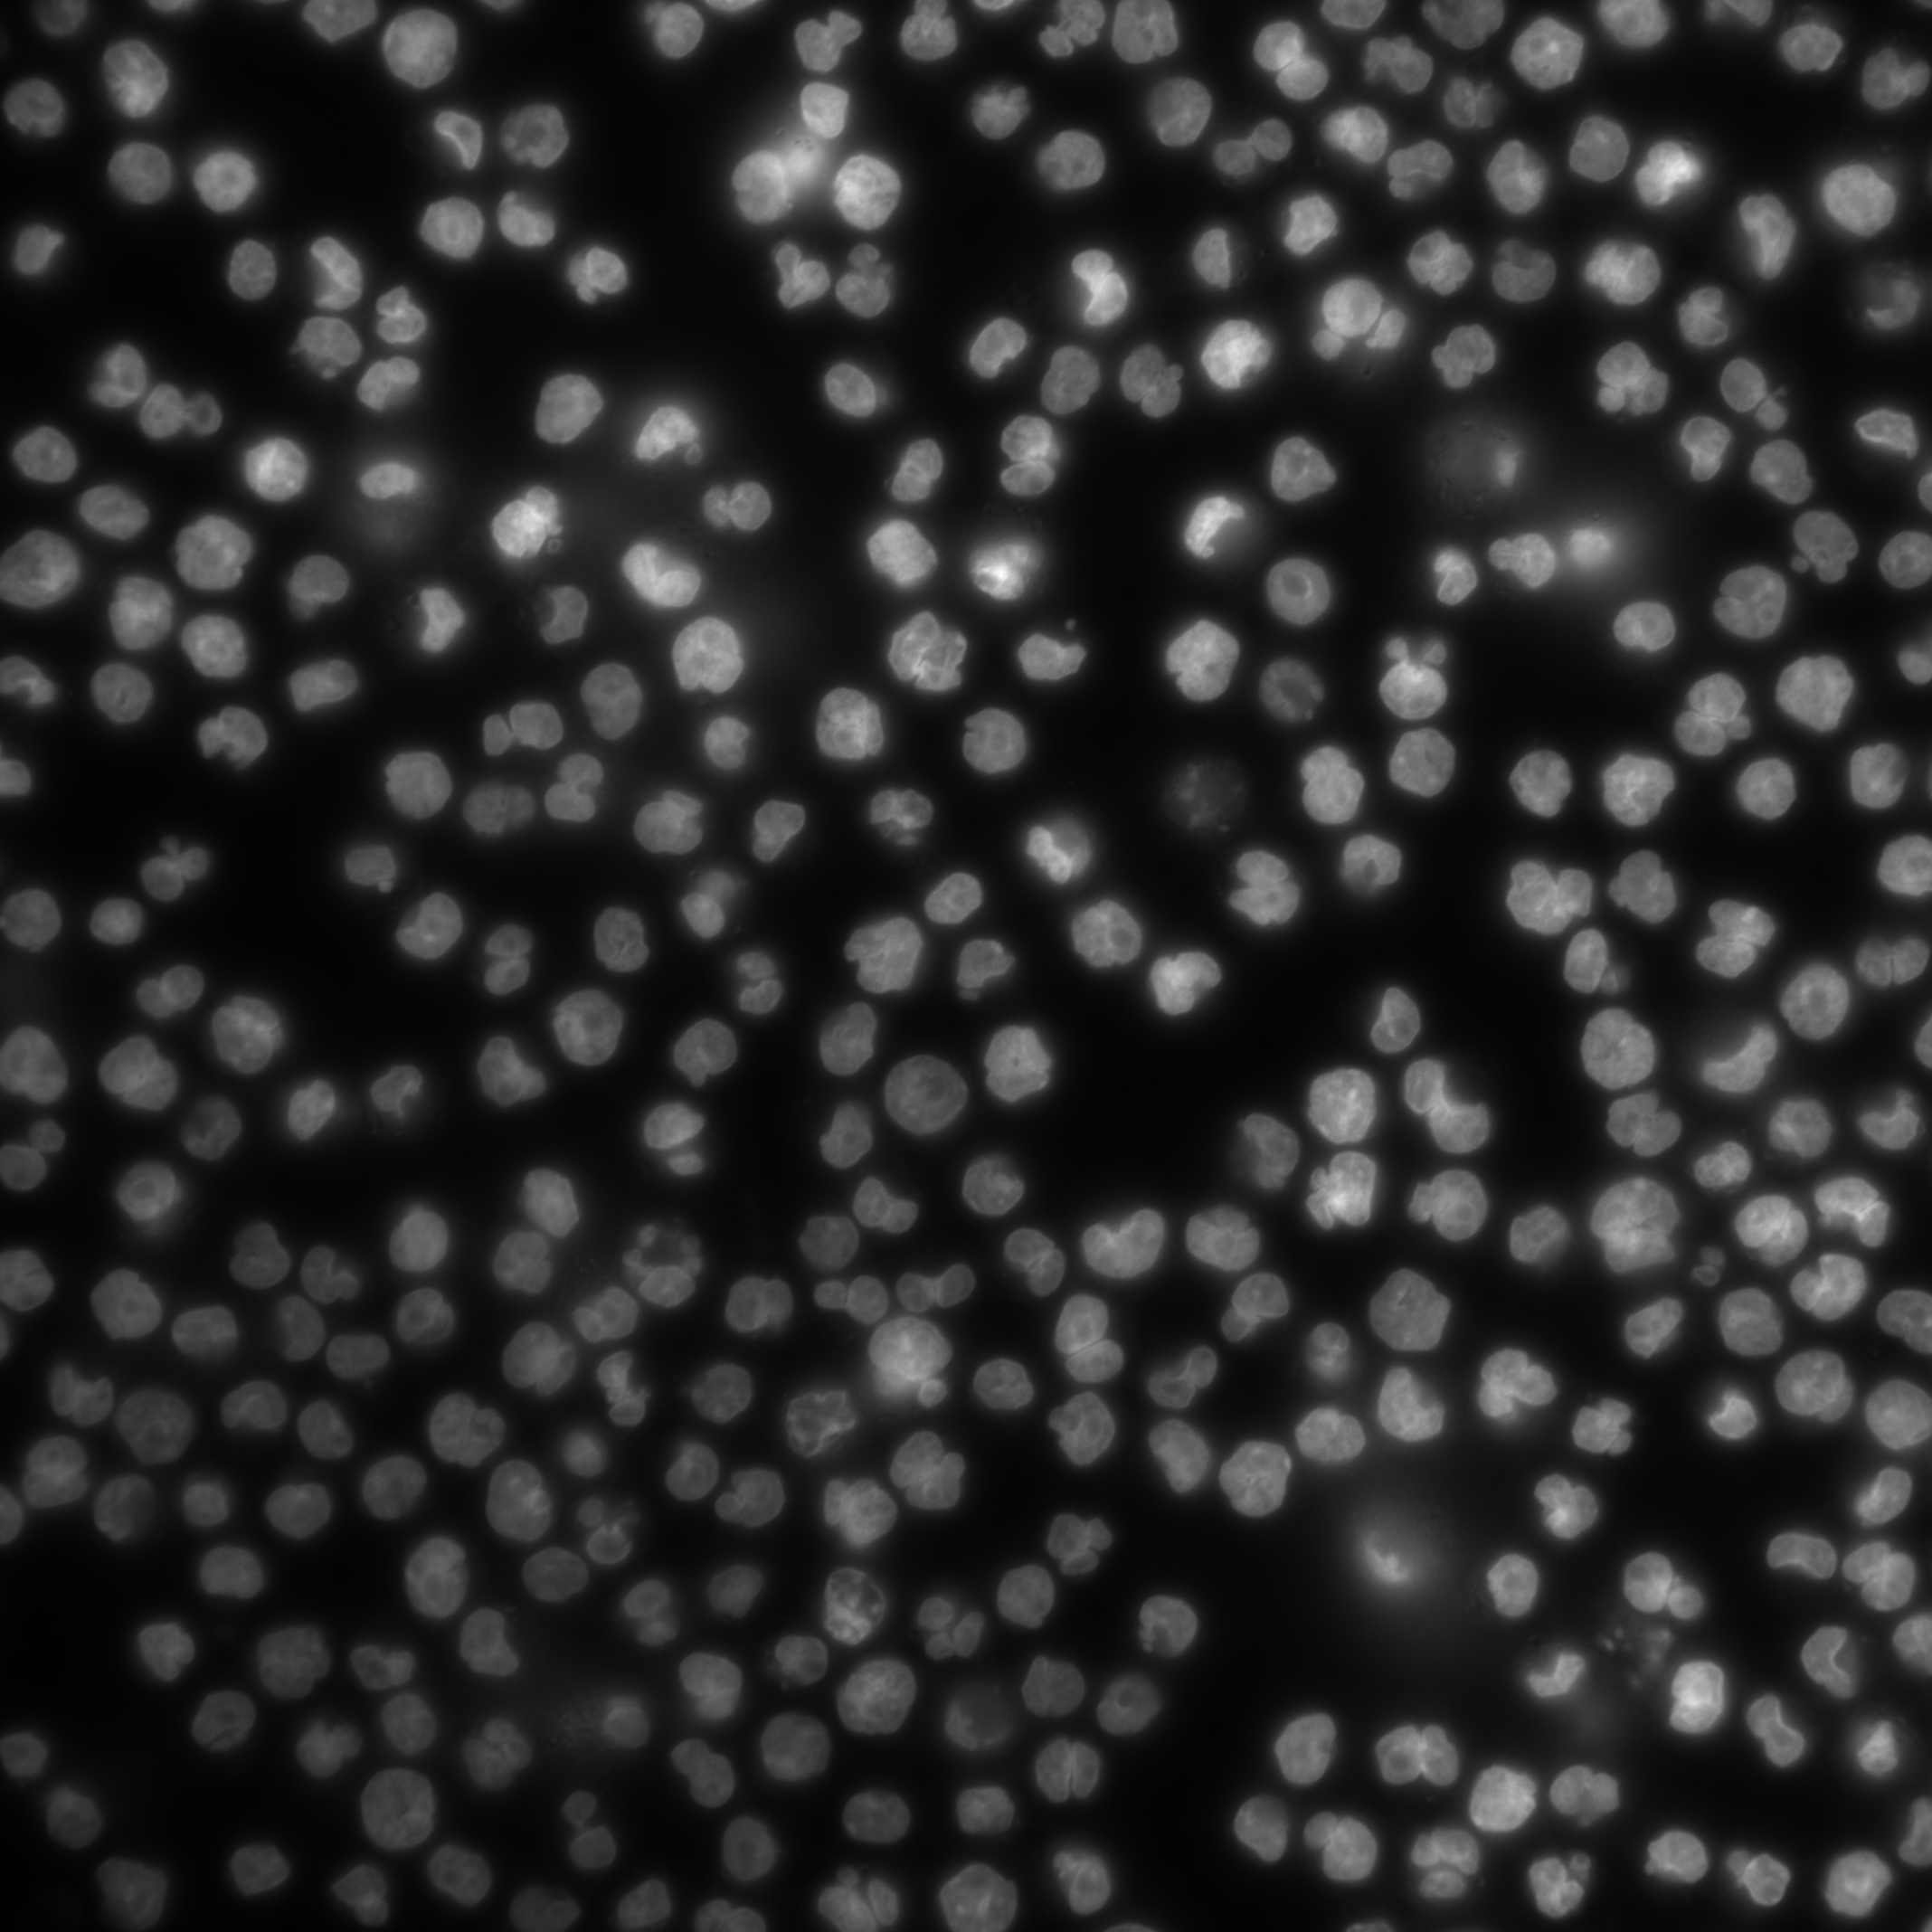
\includegraphics{bilder/lightning-conditions/lightning-3.png} &
            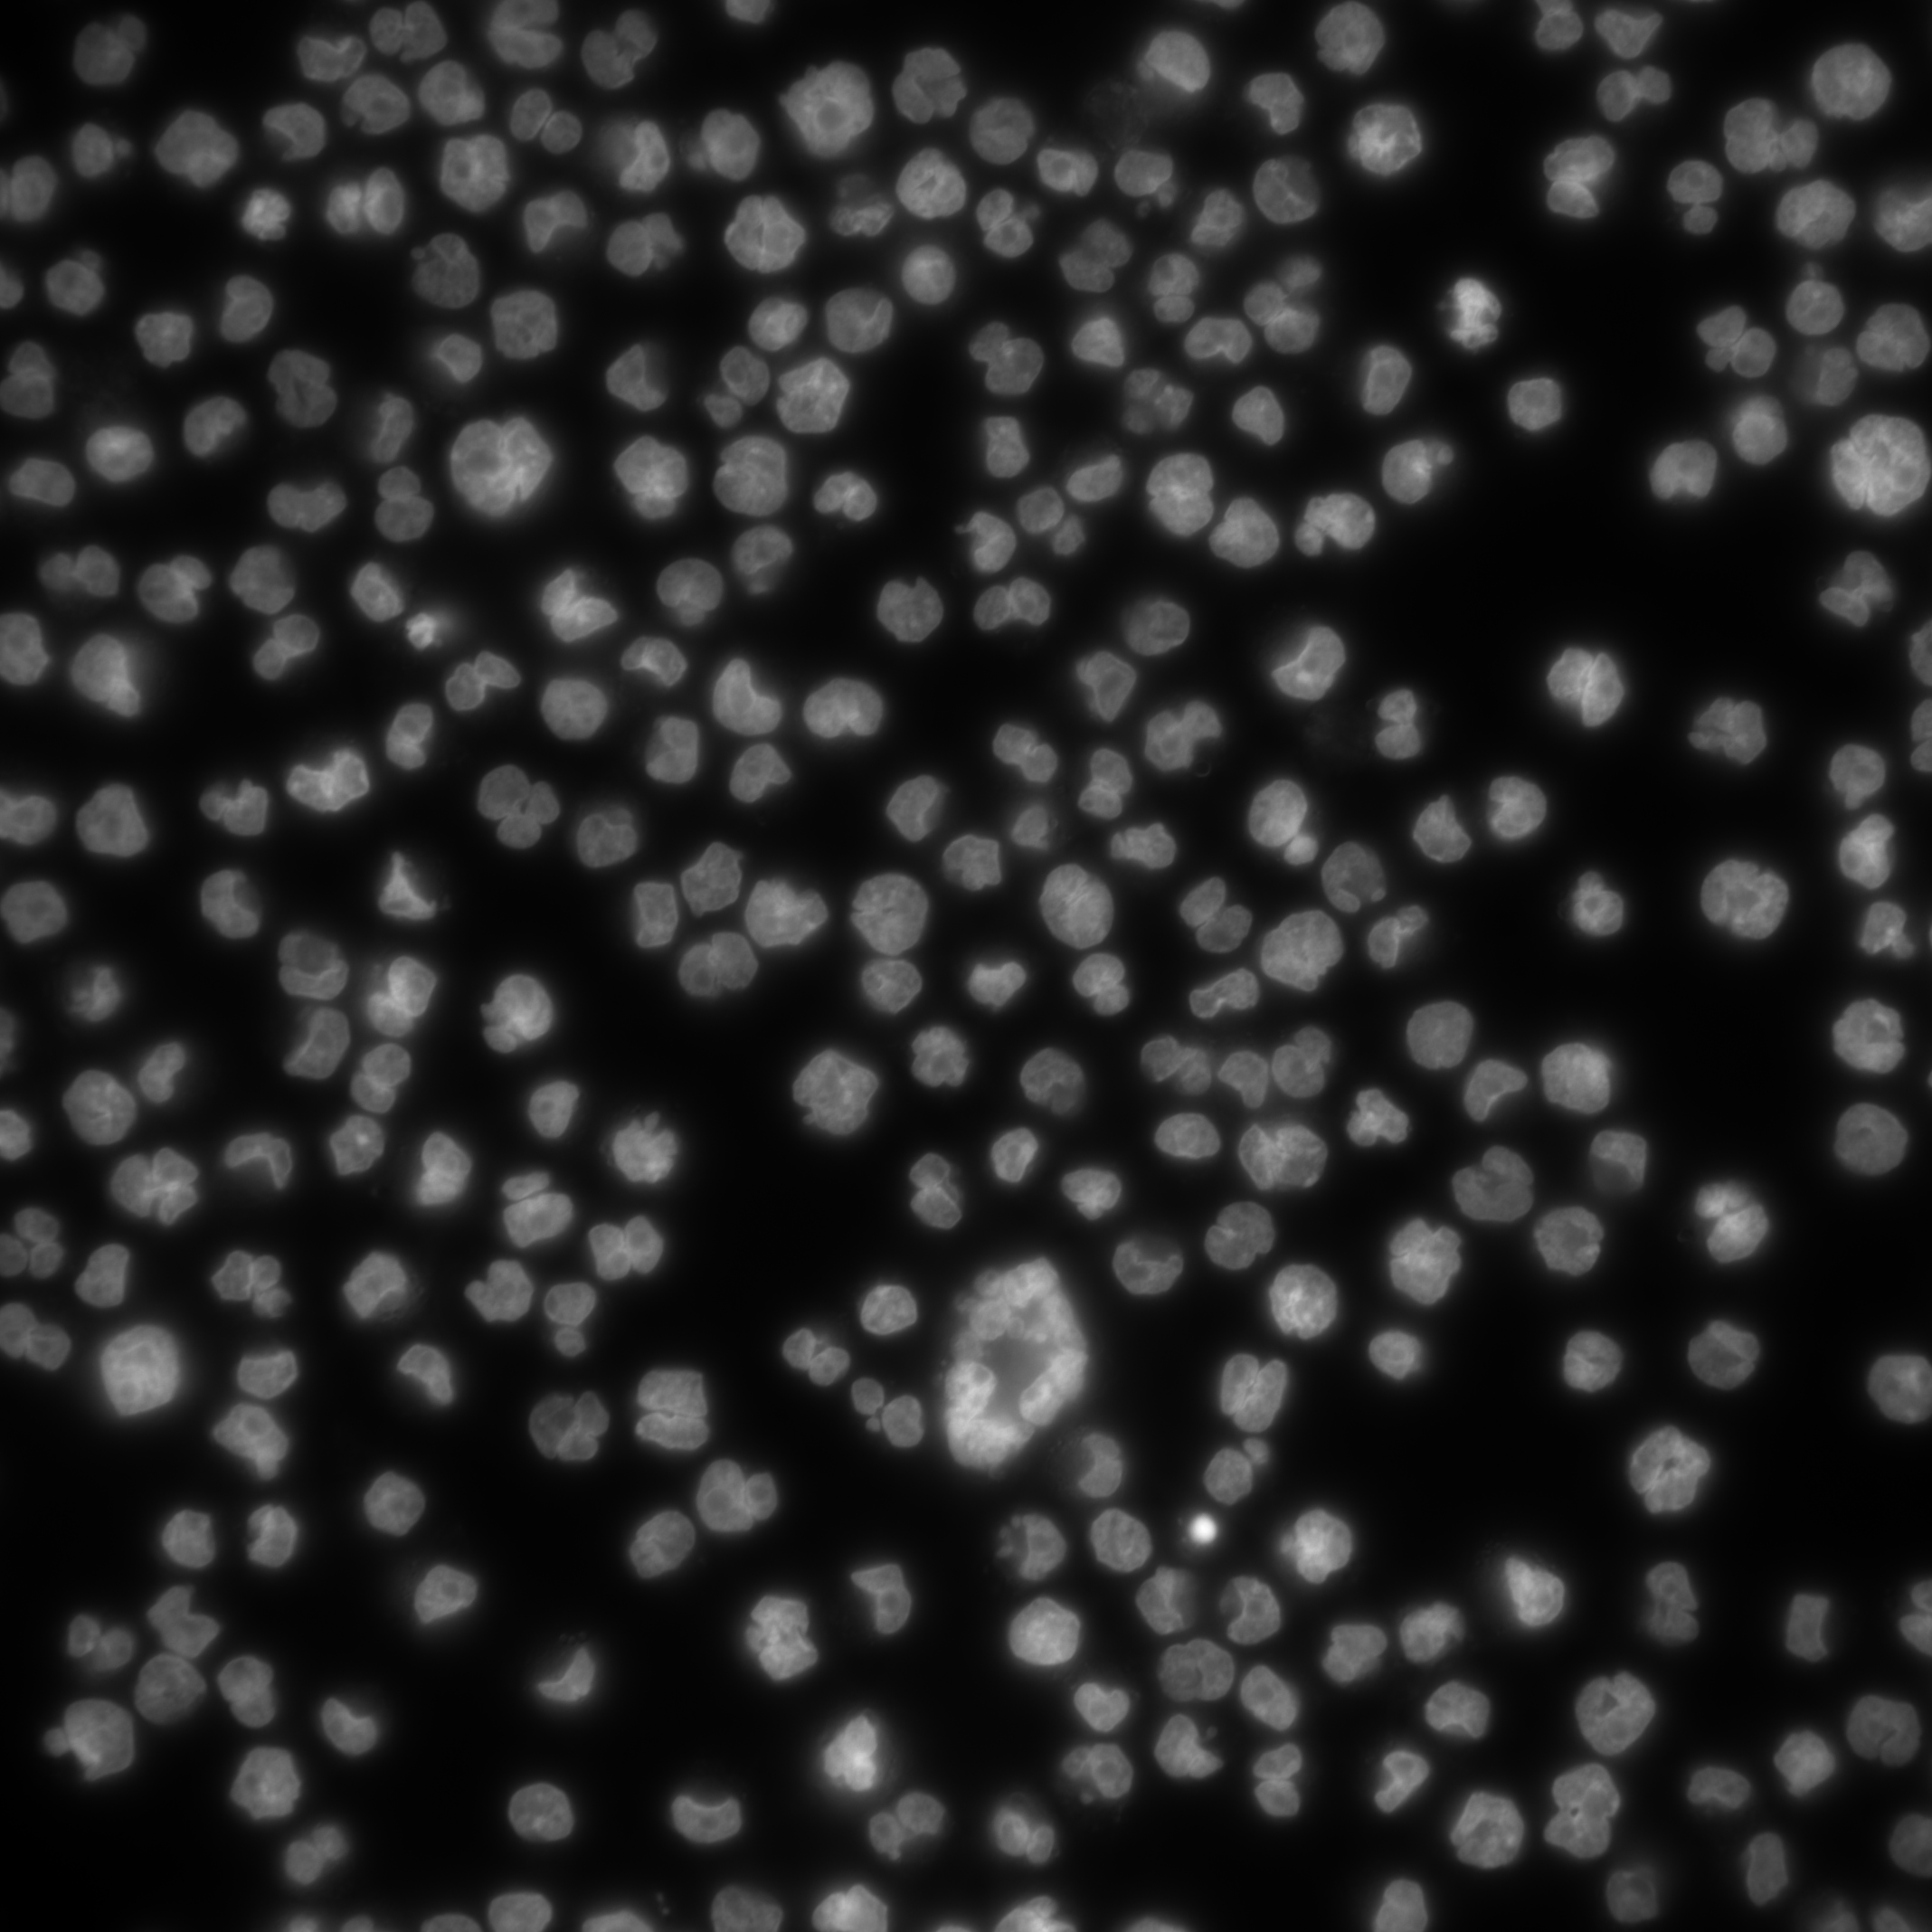
\includegraphics{bilder/lightning-conditions/lightning-4.png}
        \end{tabularx}
    \caption[Different lighting conditions]%
    {Different challenges in lightning and cells density that do not permit a successful use of a global thresholding for the foreground segmentation.}
    \label{fig:lightning_conditions}
\end{figure}

Examples of cases difficult for segmentation are presented in Figure \ref{fig:lightning_conditions} from left to right: the first image there are too few cells, which leads to the background being much darker than usual; the overexposure of one cell leads to difficulties segmenting the rest of the cells as they are hard to distinguish from the background; lighting gradient from darker (bottom left corner) to brighter (top right corner) region; normal lighting conditions.

Another challenge for segmentation bring nuclei that are very close to each other. This might happen sometimes because some of the cells are currently in the process of division. Also, when some have already fully divided, they might still be located close to one another. The example of such situations is presented in Figure \ref{fig:closely-located-cells}.

\begin{figure}[htb]
    \centering
    \subfloat[Original fluorescence]{{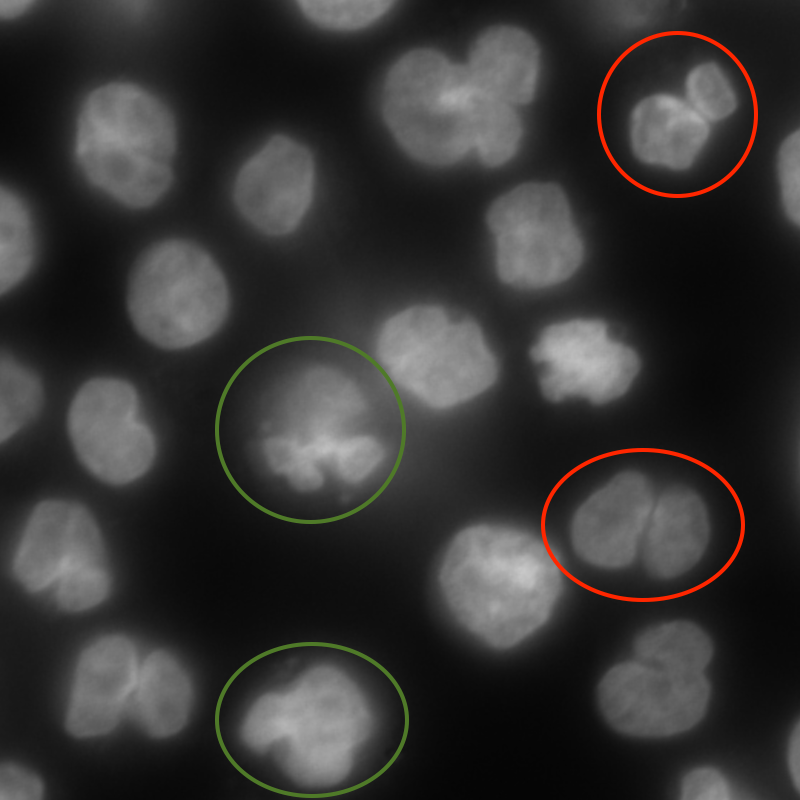
\includegraphics[width=0.2\linewidth]{bilder/close-located-cells/original.png} }}
    \qquad
    \subfloat[Segmentation (violet mask)]{{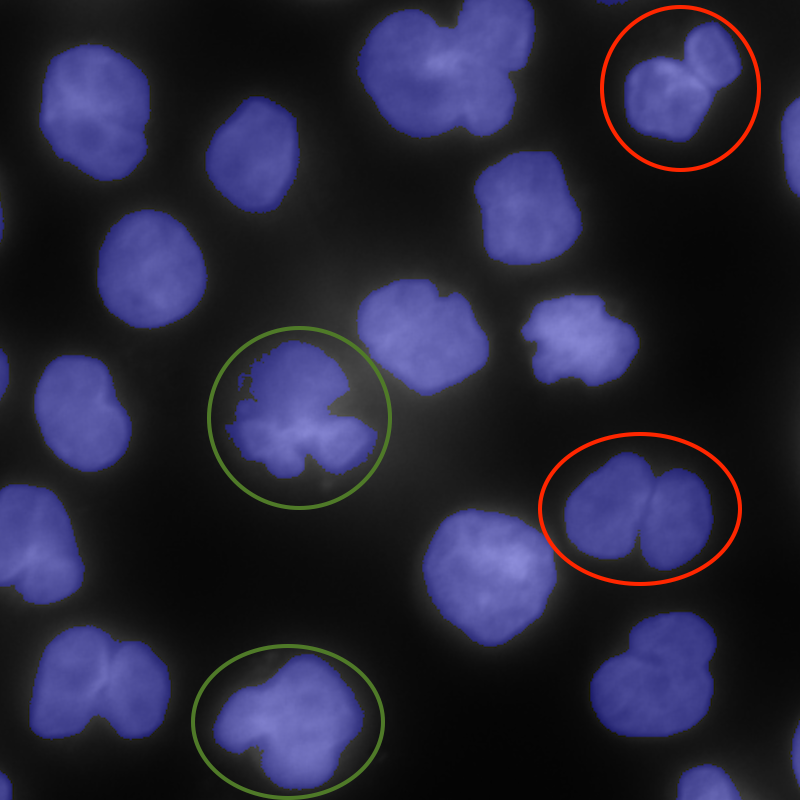
\includegraphics[width=0.2\linewidth]{bilder/close-located-cells/segmented.png} }}
    \caption[Closely located (red) and dividing (green) cells]%
    {Closely located (red) and dividing (green) cells represent a challenge for a foreground segmentation as they are recognized as one cell.}
    \label{fig:closely-located-cells}
\end{figure}

Here, the cells that are not yet fully divided are highlighted with green circles and the ones that are fully divided, but located too close to one another, are highlighted with red circles. You can see that the segmentation algorithm (see Algorithm \ref{algorithm:nuclei-segmentation}) recognises both such cases as one nucleus. This algorithm is described below and its steps are visualized in Figure \ref{fig:segmentation-nuclei-steps}.
\begin{algorithm}
    \caption{Fluorescence segmentation of nuclei}
    \begin{algorithmic}
    \item 1. Normalize image.
    \item 2. Apply local thresholding and get a threshold $T$ or a set of local thresholds \{$T_i$\} and create an initial mask: $1$ if $x_i > T$ or $0$ otherwise.
    \item 3. Apply \textit{fill\_holes} transformation to the initial mask in order to get rid of unneeded details within the nuclei.
    \item 4. Run \textit{findContours} from opencv in order to obtain separate regions and filter them based on the following criteria: filter out regions that are too big (measure the biggest possible nuclei manually), regions that are too small (measured manually as well), regions that have a shape that is not similar to convex circular type of nuclei. The last filter is done by checking the ratio of the area of the region to the area of the convex hull of the region (for more details regarding \textit{findContours} implementation refer too \cite{Suzuki_1985}).
    \end{algorithmic}
    \label{algorithm:nuclei-segmentation}
\end{algorithm}

\begin{figure}[htb]
    \centering
    \setkeys{Gin}{width=\linewidth}
    \centering
        \begin{tabularx}{\textwidth}{YYYY}
            \textbf{Normalized input} &
            \textbf{Local threshold} &
            \textbf{Filled holes} &
            \textbf{Filtered regions} \\
            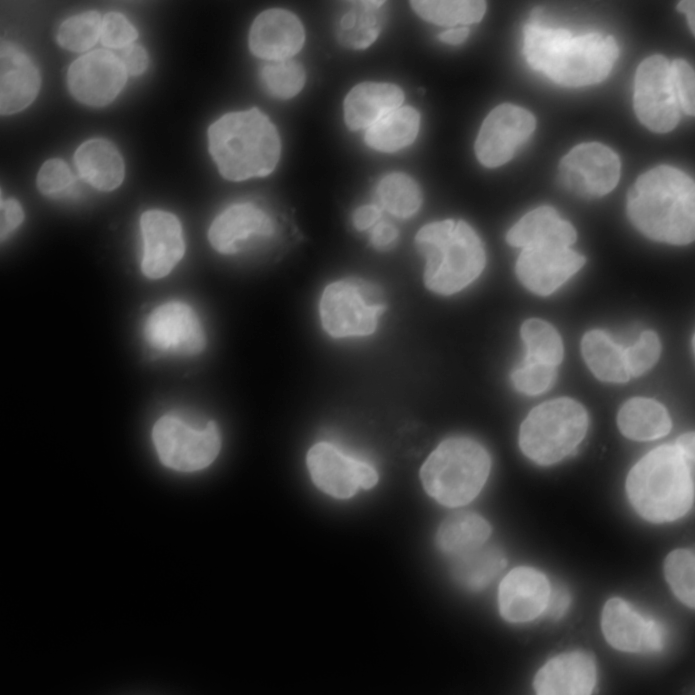
\includegraphics{bilder/segmentation/nuclei-mask/normalized.png} & 
\includegraphics{bilder/segmentation/nuclei-mask/binary_local.png} &
            
\includegraphics{bilder/segmentation/nuclei-mask/filled_holes.png} &
            
\includegraphics{bilder/segmentation/nuclei-mask/mask.png}
        \end{tabularx}
    \caption[Fluorescence segmentation]%
    {Fluorescence segmentation. Artifacts of local thresholding algorithm visible in the second image can be successfully filtered out based on their shape.}
    \label{fig:segmentation-nuclei-steps}
\end{figure}

A more detailed description of the reasoning why local thresholding approach was chosen is provided in the following subsection.

        \paragraph{Thresholding algorithms}
        There are in general two types of thresholding that exist to binarize an image (create its mask): global and local.

\textbf{Global thresholding} is a an algorithm that simply choses one threshold $T$ for the whole histogram of the image. All pixels that are smaller than this threshold $x_{i,j} < T$ are assigned to be of class $0$ (background) and all pixels that are larger than this threshold $x_{i,j} > T$ are assigned to be of class $1$ (foreground). It is very difficult to find a good threshold manually that would work out for all the images, especially in this case, when the brightness does differ not only between the images, but also within the image itself (light gradient in Figure \ref{fig:lightning_conditions}). To find a good threshold automatically (at least to some extect) \cite{digital_image_book} proposed the following algorithm:

\begin{algorithm}
  \caption{Global thresholding}
  \begin{algorithmic}
    \item 1. Select an initial estimate for $T$.
    \item 2. Segment the image using T. This will produce 2 groups of pixels $G_1$ (all pixels $x_i > T$) and $G_2$ (all pixels $x_i < T$).  
    \item 3. Computer the average gray values $\mu_1$ and $\mu_2$ for the pixels in  regions $G_1$ and $G_2$.
    \item 4. Compute a new threshold value 
        $T' = \frac{\mu_1 + \mu_2}{2}$
    \item 5. Repeat steps 2-4 until difference in the change of value $T$ is smaller that a predefined parameter.
  \end{algorithmic}
  \label{alg:global-thresholding}
\end{algorithm}

Nevertheless, it is not obvious how to preselect an initial threshold in step 1. There are several options here, however keep in mind that there is also no single best solution among them. For example, when an assumption that the foreground occupies approximately the same area as the background holds, than initial threshold $T$ should be chosen to be an average gray level and etc.

After trying out many different global threshold approaches, it has been derived that a \textit{global minimum thresholding} is the best one. It is implemented in \textit{skimage.filters} and according to the documentation (\cite{global_thresh}) works in the following way: it assumes that the histogram $p = (p_0, \ldots, p_{M})$ of the image is bimodal, meaning that it has two clearly defined peaks (background and foreground). Afetrwards the histogram is iteratively smoothed using a running average of size $k=3$. The points on the histogram are updated with the value $a_k$ from Equation \ref{eq:SMA} until only 2 local maximas ($a_l$ and $a_r$) are left. 
\begin{equation}
    a_k = \frac{1}{k}\sum_{i=n-k + 1}^{n}p_i
\label{eq:SMA}
\end{equation}
Then the threshold is taken as the minimum between the two local maximas:
\begin{equation}
    a_l \leq T \leq a_r
\end{equation}

One clear downside of this approach though is that images which histograms have very unequal peaks or a broad and flat valley will be unsuitable for this method (\cite{thresholding_skimage}).

\begin{figure}[htb]
	\begin{center}
		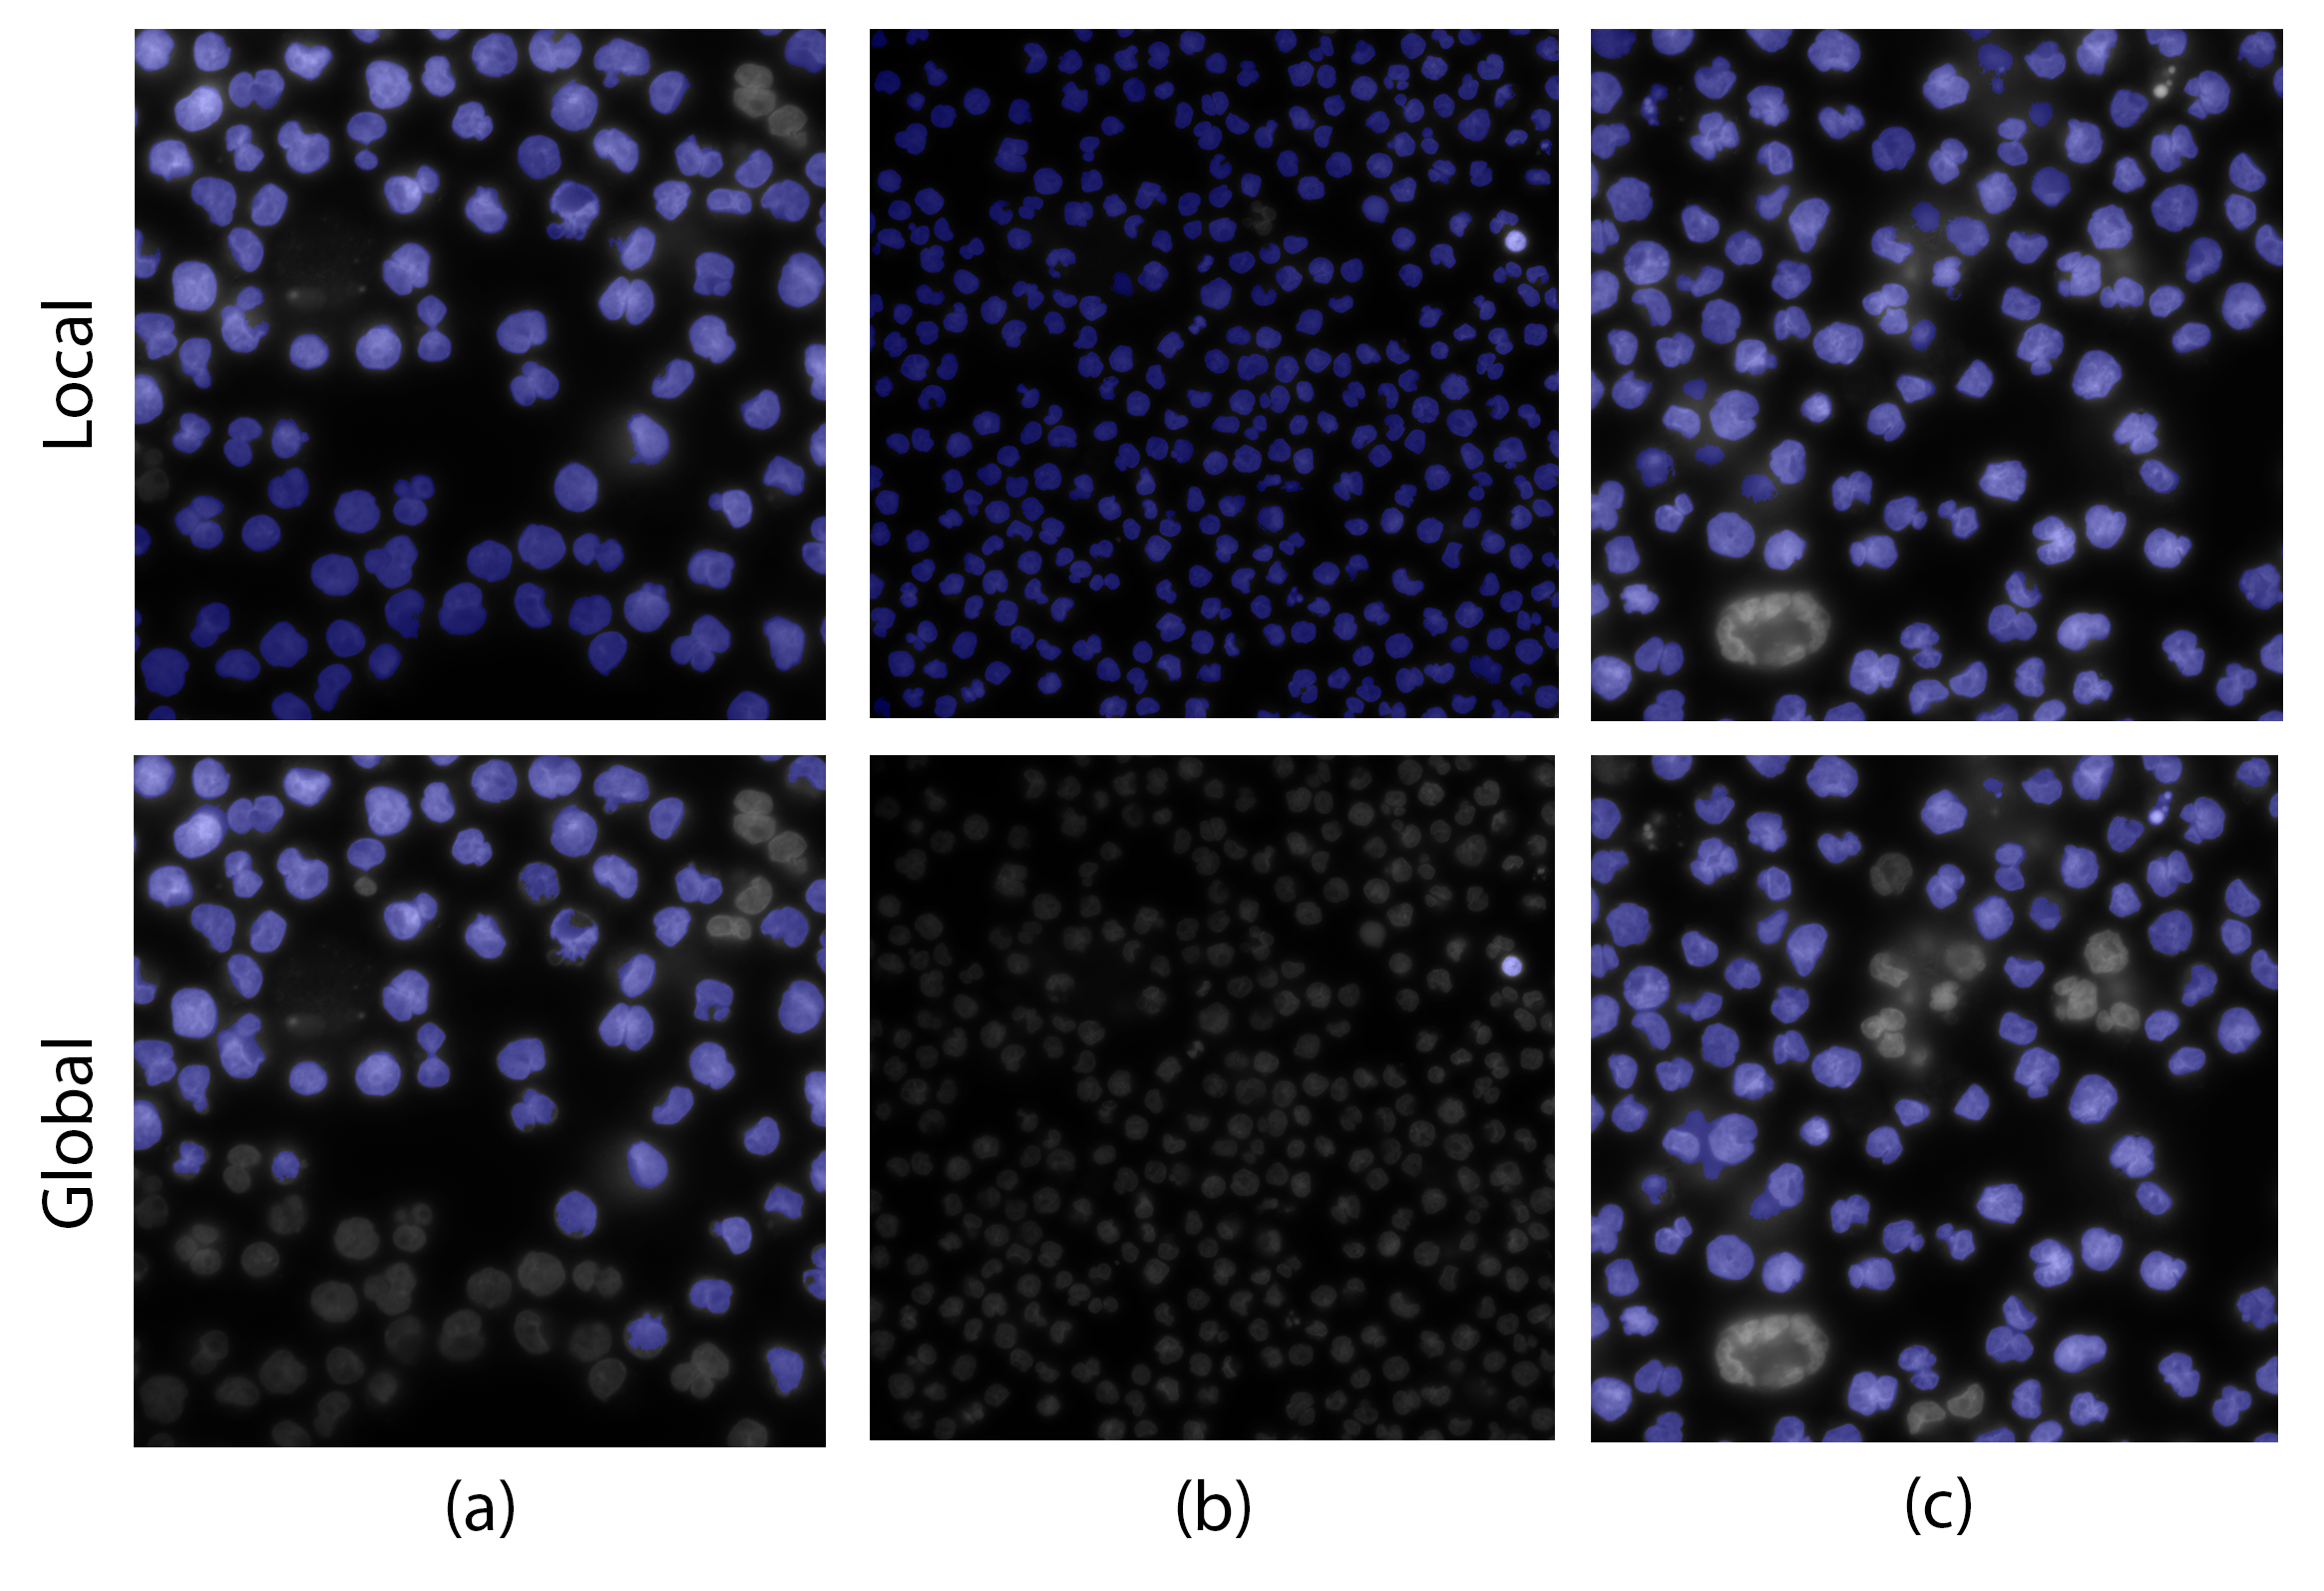
\includegraphics[width=0.6\linewidth]{bilder/difficult-lightning/local-vs-global.png}
		\caption{Local vs. global thresholding}\label{fig:thresholding-bad-conditions}
	\end{center}
\end{figure}

Unfortunately this method did not perfom well even for the images that have an equal amount of foreground and background. And the reason for that is a mentioned above non-uniform illumination within the images. For visual comparison of global thresholding applied to difficult images see Figure \ref{fig:thresholding-bad-conditions}a, b, c Global. \ref{fig:thresholding-bad-conditions}c is an image with equal brightness level, however even there some mistakes do appear.

However there is another better approach that performs well in such conditions: \textbf{local thresholding}. For nuclei segmentation exactly this algorithm was chosen. It is implemented in \textit{skimage.filters} and can be used in the following way:

\begin{lstlisting}
  skimage.filters.local_threshold(img, block_size=7, method='gaussian', offset=0)
\end{lstlisting}

The main idea behind it is the following: instead of selecting one threshold for the whole image (global one), one can select several thresholds for each local region with a predefined size. The comparison between global and local thresholding is presented in Figure \ref{fig:thresholding-bad-conditions}, where (a), (b) denote exteme corruption cases and (c) represents a normal illumination.

"The threshold value is the weighted mean for the local neighborhood of a pixel subtracted by a constant (\cite{digital_image_book})". With the image size of $2136 \times 2136$, the local neighborhood (or a \textit{block\_ size}) by experimenting with different values was chosen equal to $111$. The default \textit{method} used on for local thresholding is \textit{gaussian}, \textit{offset} value is a constant that will be subtracted from weighted mean of neighborhood during the calculation of the local threshold, by default this value is $0$ \cite{local_thresholding}.

Let $z$ be a random variable that quantifies a gray-level value of the pixel, then the histogram of the image is a probability density function (PDF) $p(z)$. Since we assume that the image contains a background and a foreground, then this PDF is a mixture of two densities $p_1(z)$ and $p_@(z)$ weighted by the relative areas of these two classes (their number of pixels) $P_1$ and $P_2$. Then 

\begin{equation}
    p(z) = P_1 p_1(z) + P_2 p_2(z)
\end{equation}

By assuming Gauassian model for both $p_1(z)$ and $p_2(z)$, one gets a Gaussian Mixture Model (GMM). Since we have assumed that each pixel can be asssigned to either a background of foreground only, $P_1 + P_2 = 1$ must hold. 

\begin{figure}[htb]
	\begin{center}
		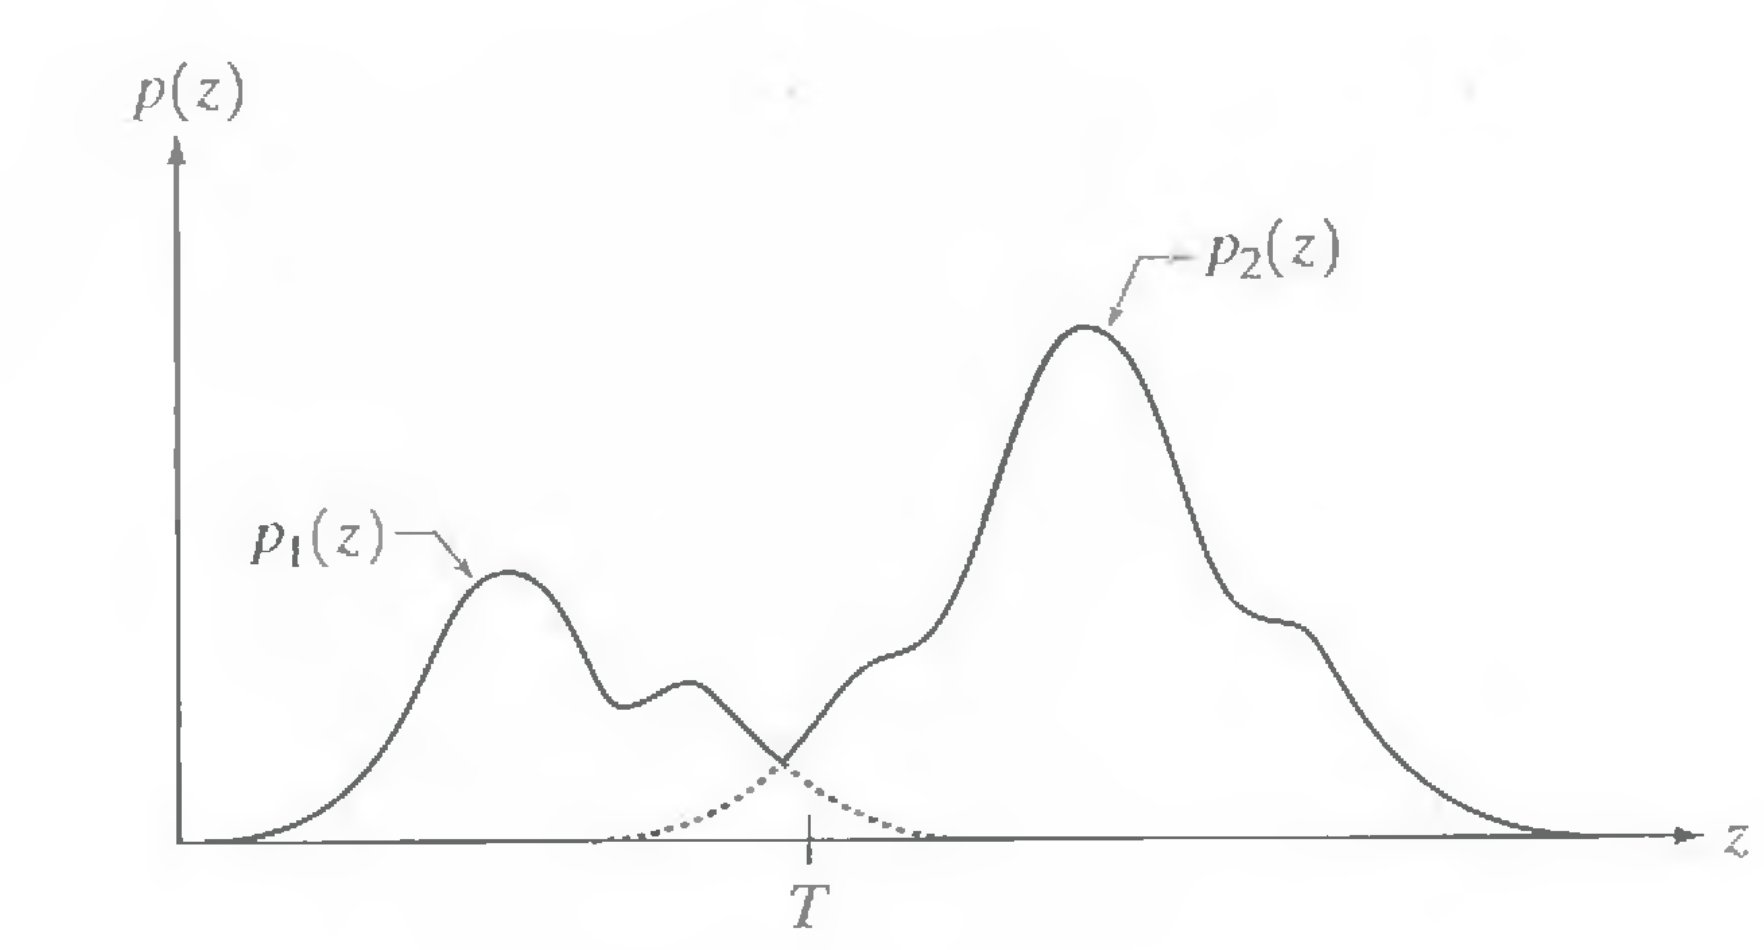
\includegraphics[width=0.8\linewidth]{bilder/Gonzalez.png}
		\caption{Histogram as a probability density function (\cite{digital_image_book})}\label{fig:gmm}
	\end{center}
\end{figure}

Probability to falsely classify an background pixel as a foreground then is:

\begin{equation}
    E_1(T) = \int_{-\infty}^T{p_2(z) \, dz}
\end{equation}

And probability to falsely classify a foreground pixel as a background then is:

\begin{equation}
    E_2(T) = \int_T^{+\infty}{p_1(z) \, dz}
\end{equation}

The overall error is:

\begin{equation}
    E(T) = P_1E_1(T) + P_2E_2(T)
\end{equation}

By differentiating $E(T)$ wrt. to $T$ and equating the result to zero the optimal solution will be:

\begin{equation}
    P_1p_1(T) = P_2p_2(T)
\end{equation}

Since Gaussian distributions have been assumed, it will hold that:
\begin{equation}
    p(z) = \frac{P_1}{\sqrt{2\pi} \sigma_1}e^{-\frac{(z-\mu_1)^2}{2\sigma_1^2}} + \frac{P_2}{\sqrt{2\pi} \sigma_2}e^{-\frac{(z-\mu_2)^2}{2\sigma_2^2}}
\end{equation}

With $\mu_i$ and $\sigma_i^2$ for $i \in \{1, 2\}$ being the mean and variance of the Gaussian distribution $p_i(z)$. This results in the following solution for $T$:
\begin{equation}
    \begin{split}
        &AT^2 + BT + C = 0 \\
        &A = \sigma_1^2 + \sigma_2^2 \\
        &B = 2(\mu_1 \sigma_1^2 - \mu_2 \sigma_2^2) \\
        &C = \sigma_1^2 \mu_2^2 - \sigma_2^2 \mu_1^2 + 2\sigma_1^2 2\sigma_2^2ln\left(\frac{\sigma_2P_1}{\sigma_1P_2}\right)
    \end{split}
\end{equation}

To escape two optimal solutions of the quadratic equation, it may be assumed that $\sigma_1 = \sigma_2 = \sigma$ and then:

\begin{equation}
    T = \frac{\mu_1 + \mu_2}{2} + \frac{\sigma^2}{\mu_1 - \mu_2}ln\left(\frac{P_2}{P_1}\right)
\end{equation}

Such threshold search is then applied to all of the subregions of the image with overlaps. Thresholds are calculated only for the regions that contain two clear peaks in their histograms and interpolated to the other pixels from the regions that do not contain them. If the subregions does not contain two peaks, it simply means that there is no foreground or background object on it. 

\begin{table}[htb]
  \centering
      \begin{tabular}{||c c||} 
       \hline
       Local Threshold & Global Threshold \\ [0.5ex] 
       \hline\hline
       0.3 sec & 17 sec  \\ 
       \hline
      \end{tabular}
      \caption{Threshold timing}
      \label{table:threshold-timing}
  \end{table}
  
Of course local thresholding approach has a longer runtime time (see Table \ref{table:threshold-timing}). Therefore when the inference speed is crutial one can still use \textit{global minimum thresholding}. It does performs visually a bit worse that a local threshold (especially for the extreme corrupted cases), however for the normal conditions the performance is quite similar ot the local thresholding (Figure \ref{fig:thresholding-bad-conditions}c).



    \subsubsection{Biological metrics}
        In this subsection the evaluation of the model trained on full nuclei dataset with full set of augmentations is presented. Distributions of number of nuclei and their area are very similar in shape, the corresponding scatter plots form almost linear dependance. Distributions of intensities are less similar, the higher intensity of predicted images is proved here. However, high scores in Pearson and Spearman correlation coefficients (see Table \ref{table:nuclei-downstream-metrics-coefficients}) suggest that distributions are indeed close to each other. The difference between predictions and ground truth might be caused by an absolute value shift, that can be easily fixed.
\begin{figure}[htb]
	\begin{center}
		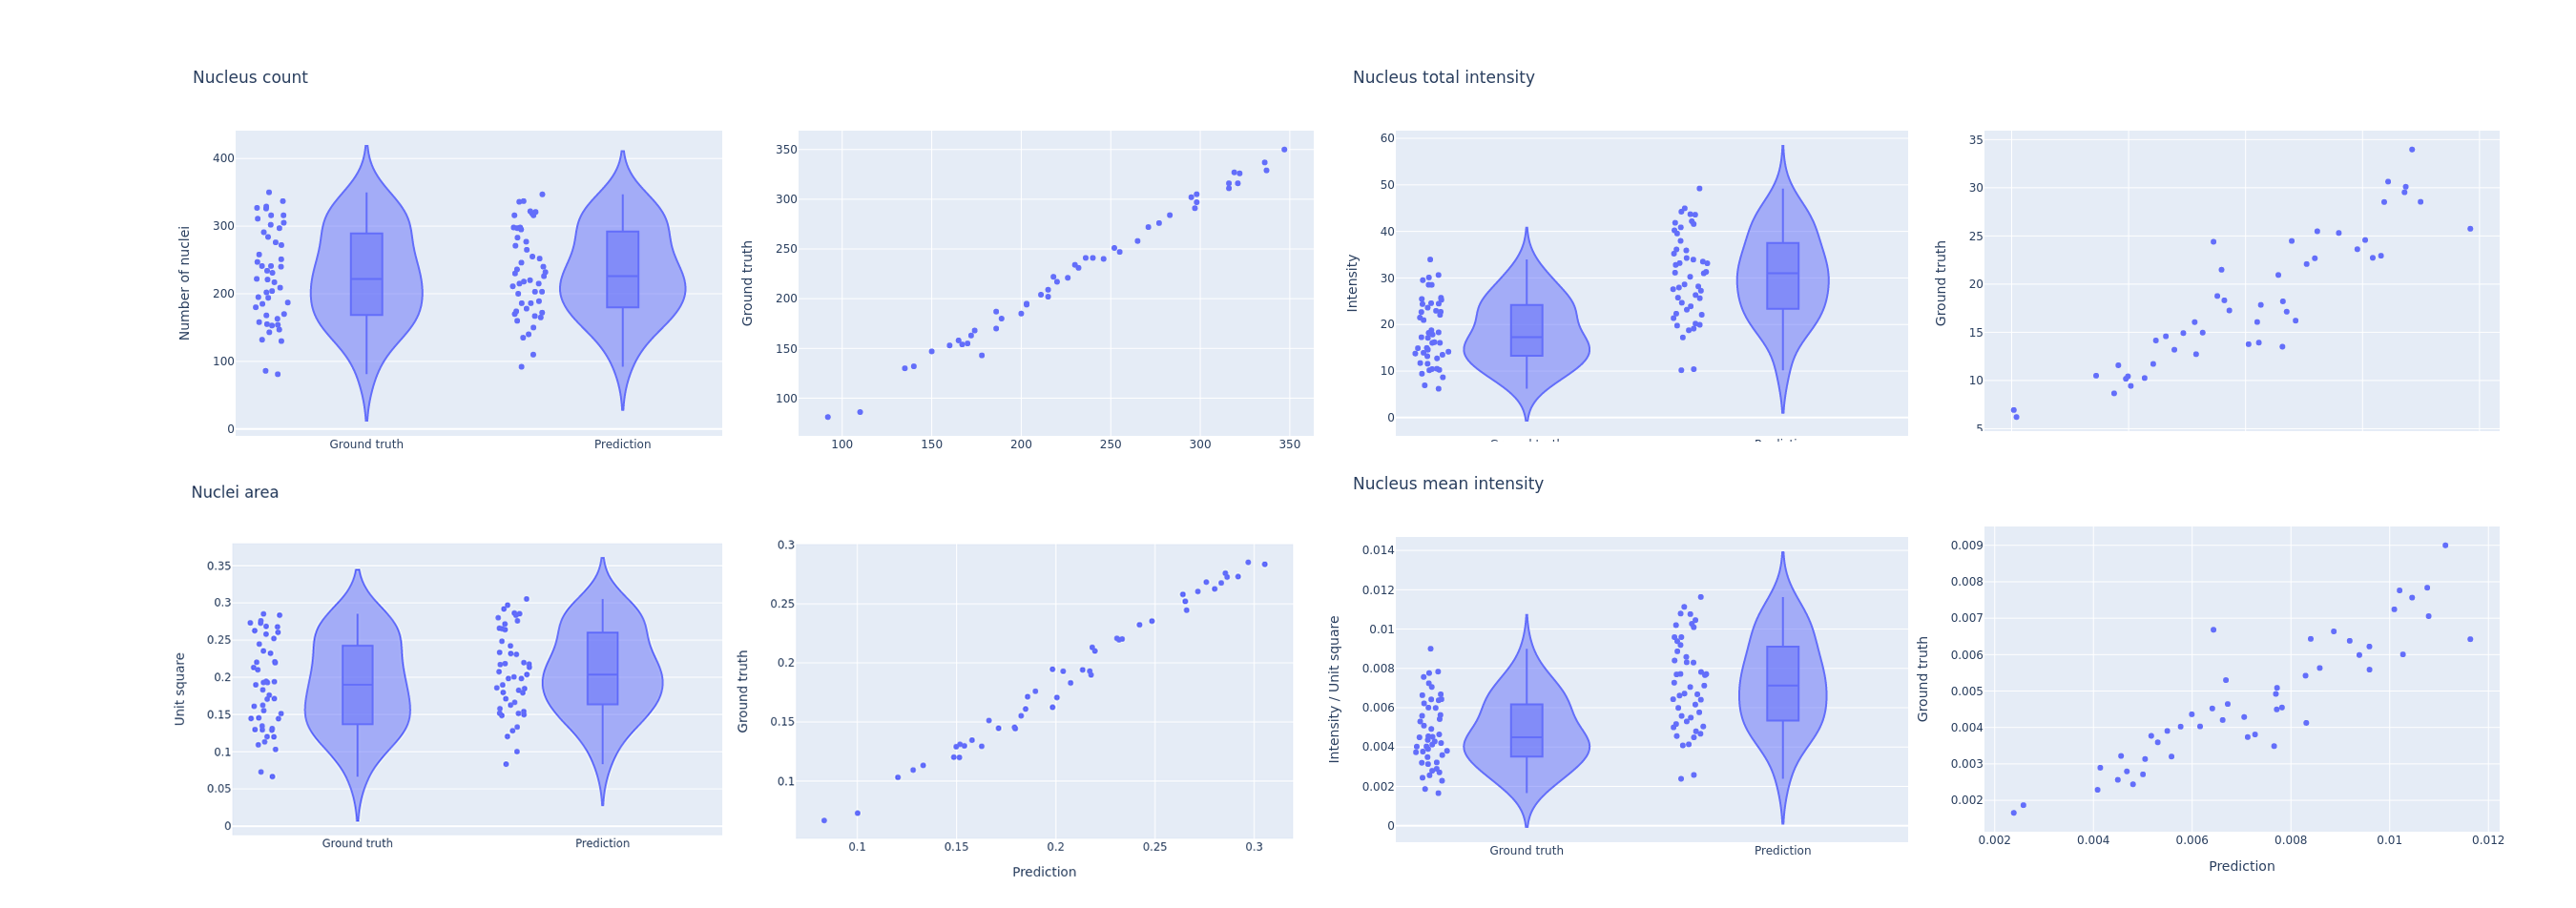
\includegraphics[width=\linewidth]{bilder/nuclei/metric/combined-metrics.png}
		\caption{Metrics for downstream tasks on nuclei}\label{fig:nuclei-downstream-metrics}
	\end{center}
\end{figure}

\begin{table}[htb]
    \centering
    \caption{Correlation coefficients for downstream tasks on nuclei}
        \begin{adjustbox}{width=0.4\textwidth}
            \begin{tabular}{|c|c|c|}\hline
                &Pearson&Spearman
                \\\hline\hline
                Number of nuclei&0.995&0.994\\\hline
                Total intensity&0.902&0.911\\\hline
                Mean intensity&0.907&0.904\\\hline
                Area&0.992&0.990\\\hline
            \end{tabular}
        \label{table:nuclei-downstream-metrics-coefficients}
        \end{adjustbox}
\end{table}

    \subsubsection{Influence of scaling on predictions quality}
        Examples of predictions quality with different scales.

\begin{table}[H]
    \centering
    \caption{Paerson correlation coefficients for downstream tasks for different scaling factors} 
        \begin{adjustbox}{width=\textwidth}
            \begin{tabular}{|M{35mm}|M{35mm}|M{35mm}|M{35mm}|M{35mm}|M{35mm}|M{35mm}|}\hline
                &1.3 scale&0.7 scale&Train (1.0 scale + augments) \newline Predict (1.3 scale)&Train (1.3 scale) \newline Predict (1.0 scale)&Train (1.3 scale) \newline Predict (0.7 scale)
                \\\hline\hline
                Number of nuclei&0.987&0.995&0.975&0.971&?\\\hline
                Total intensity&0.902&.88&0.861&0.856&?\\\hline
                Mean intensity&0.922&0.906&0.88&0.872&?\\\hline
                Area&0.991&0.992&0.961&0.952&?\\\hline
            \end{tabular}
        \end{adjustbox}
\end{table}

    \subsubsection{Conclusions}
        Fluorescence staining of nucleus in CHO cells used for recombinant protein production at Merck KGaA can be successfully replaced with \textit{in silico} labeling using deep a neural network. The provided dataset is big enough to achieve accurate predictions, nevertheless further research could be dedicated to improving fluorescence image preprocessing in order to remove blur around the nucleus, as well as to cleaning the data from the under- or overexposed images.

The model successfully converges, and the use of augmentations improves its performance. Pearson correlation coefficient is more representative for the model's predictions evaluation than MSE, and MSE is not representative of a model's quality in this case. The performance of a model is evaluated in terms of practical biological metrics. Further research can also be conducted to advance the architecture of the model, as the use of more parameters improved the predictions significantly both visually and in metrics.

In order to perform segmentation of the nucleus it is recommended to use a local thresholding approach when the inference time is not crucial and global minimum thresholding algorithm when the inference time is critical. Training the model on cells of a larger size slightly improves the intensity predictions. Yet a slight change in cell size does not influence the model's performance significantly.

